% ============================================================
%  Constraint Before Content:
%  A Mathematical Roadmap Toward the Study of
%  Structure-Preserving Transformations and Field Theory
%
%  Flyxion --- Independent Researcher
%  First Edition, 2026
% ============================================================

\documentclass[12pt, twoside, openright, a4paper]{book}

\usepackage{fontspec}
\usepackage{microtype}
\usepackage{amsmath, amssymb, amsthm, mathtools}
\usepackage{stmaryrd}
\setmainfont{TeX Gyre Pagella}
\setsansfont{TeX Gyre Heros}[Scale=MatchLowercase]

\usepackage[dvipsnames, svgnames, table]{xcolor}
\definecolor{RSVPdeep}{HTML}{0D3349}
\definecolor{RSVPmid}{HTML}{1A5276}
\definecolor{RSVPlight}{HTML}{D6EAF8}
\definecolor{RSVPaccent}{HTML}{E67E22}
\definecolor{RSVPwarm}{HTML}{FDF2E9}
\definecolor{RSVPgray}{HTML}{F4F6F7}
\definecolor{RSVPgreen}{HTML}{1E8449}
\definecolor{RSVPpurple}{HTML}{6C3483}

\usepackage[a4paper, top=25mm, bottom=30mm, inner=30mm, outer=22mm,
  marginparwidth=14mm, marginparsep=3mm, headsep=8mm]{geometry}

\usepackage{fancyhdr}
\setlength{\headheight}{24pt}
\pagestyle{fancy}
\fancyhf{}
\fancyhead[LE]{\small\color{RSVPmid}\scshape\leftmark}
\fancyhead[RO]{\small\color{RSVPmid}\scshape\rightmark}
\fancyfoot[LE,RO]{\color{RSVPaccent}\bfseries\thepage}
\fancyfoot[CO,CE]{\small\color{RSVPmid!60}Constraint Before Content --- Flyxion}
\renewcommand{\headrulewidth}{0.4pt}
\renewcommand{\headrule}{\hbox to\headwidth{\color{RSVPmid}\leaders\hrule height\headrulewidth\hfill}}

\usepackage{titlesec}
\titleformat{\part}[display]
  {\centering\color{RSVPdeep}\Huge\bfseries}
  {\color{RSVPaccent}\scshape\large Part \thepart}{1em}{}
\titleformat{\chapter}[display]
  {\color{RSVPdeep}\huge\bfseries}
  {\hfill\colorbox{RSVPdeep}{\color{white}\fontsize{36}{36}\selectfont\quad\thechapter\quad}}
  {0.5em}{\rule{\linewidth}{1.5pt}\vspace{0.3em}\\}
\titlespacing{\chapter}{0pt}{-20pt}{40pt}
\titleformat{\section}{\color{RSVPdeep}\Large\bfseries}{\color{RSVPaccent}\thesection}{0.8em}{}
\titleformat{\subsection}{\color{RSVPmid}\large\bfseries}{\thesubsection}{0.7em}{}

\usepackage[most, hooks, skins, breakable]{tcolorbox}
\tcbuselibrary{theorems, skins}
\tcbset{defstyle/.style={
  enhanced, breakable, colback=RSVPwarm, colframe=RSVPaccent,
  coltitle=white, fonttitle=\bfseries\sffamily,
  attach boxed title to top left={yshift=-2mm, xshift=6mm},
  boxed title style={colback=RSVPaccent, colframe=RSVPaccent, sharp corners},
  sharp corners=south, arc=4pt, boxrule=0.8pt,
  top=4mm, left=4mm, right=4mm, bottom=4mm}}
\newtcbtheorem[number within=chapter]{definition}{Definition}{defstyle}{def}
\newtcbtheorem[number within=chapter]{theorem}{Theorem}{
  enhanced, breakable, colback=RSVPlight, colframe=RSVPdeep,
  coltitle=white, fonttitle=\bfseries\sffamily,
  attach boxed title to top left={yshift=-2mm, xshift=6mm},
  boxed title style={colback=RSVPdeep, sharp corners},
  sharp corners=south, arc=4pt, boxrule=1pt,
  top=4mm, left=4mm, right=4mm, bottom=4mm}{thm}
\newtcbtheorem[number within=chapter]{proposition}{Proposition}{
  enhanced, breakable, colback=RSVPlight!60, colframe=RSVPmid,
  coltitle=white, fonttitle=\bfseries\sffamily,
  attach boxed title to top left={yshift=-2mm, xshift=6mm},
  boxed title style={colback=RSVPmid, sharp corners},
  sharp corners=south, arc=4pt, boxrule=0.8pt,
  top=4mm, left=4mm, right=4mm, bottom=4mm}{prop}
\newtcolorbox{examplebox}[1][]{
  enhanced, breakable, colback=RSVPgray, colframe=RSVPmid!50,
  coltitle=RSVPdeep, fonttitle=\bfseries\sffamily, title={Example},
  attach boxed title to top left={yshift=-2mm, xshift=4mm},
  boxed title style={colback=RSVPgray, colframe=RSVPmid!50},
  arc=4pt, boxrule=0.5pt, top=4mm, left=4mm, right=4mm, bottom=4mm, #1}
\newtcolorbox{conceptaside}[2][]{
  enhanced, breakable, colback=RSVPpurple!8, colframe=RSVPpurple!60,
  coltitle=white, fonttitle=\bfseries\sffamily, title={Conceptual Aside: #2},
  attach boxed title to top left={yshift=-2mm, xshift=6mm},
  boxed title style={colback=RSVPpurple!80, sharp corners},
  arc=6pt, boxrule=0.6pt, top=5mm, left=5mm, right=5mm, bottom=5mm, #1}
\newtcolorbox{historynote}[1][]{
  enhanced, breakable, colback=Sepia!8, colframe=Sepia!50,
  borderline west={3pt}{0pt}{Sepia!70}, sharp corners, boxrule=0pt,
  left=8mm, right=4mm, top=3mm, bottom=3mm,
  fonttitle=\bfseries\sffamily\color{Sepia!80},
  title={Historical Note}, attach title to upper={\\[1mm]}, #1}
\newtcolorbox{remarkbox}[1][]{
  enhanced, breakable, colback=white, colframe=RSVPpurple,
  borderline west={3pt}{0pt}{RSVPpurple}, sharp corners, boxrule=0pt,
  left=8mm, right=4mm, top=3mm, bottom=3mm,
  fonttitle=\bfseries\sffamily\color{RSVPpurple},
  title={$\star$ Remark}, attach title to upper={\\[1mm]}, #1}
\newtcolorbox{motivation}{
  enhanced, breakable, colback=RSVPdeep!6, colframe=RSVPdeep!40,
  coltitle=white, fonttitle=\bfseries\sffamily, title={Motivation},
  attach boxed title to top left={yshift=-2mm, xshift=6mm},
  boxed title style={colback=RSVPdeep!60, sharp corners},
  arc=4pt, boxrule=0.6pt, top=4mm, left=5mm, right=5mm, bottom=4mm,
  before upper={\parindent=0pt}}
\newtcolorbox{structures}{
  enhanced, breakable, colback=RSVPaccent!6, colframe=RSVPaccent!50,
  coltitle=white, fonttitle=\bfseries\sffamily, title={Structures Introduced},
  attach boxed title to top left={yshift=-2mm, xshift=6mm},
  boxed title style={colback=RSVPaccent!80, sharp corners},
  arc=4pt, boxrule=0.6pt, top=4mm, left=5mm, right=5mm, bottom=4mm,
  before upper={\parindent=0pt}}
\newtcolorbox{dependencies}{
  enhanced, breakable, colback=RSVPpurple!6, colframe=RSVPpurple!40,
  coltitle=white, fonttitle=\bfseries\sffamily, title={What Depends on This},
  attach boxed title to top left={yshift=-2mm, xshift=6mm},
  boxed title style={colback=RSVPpurple!70, sharp corners},
  arc=4pt, boxrule=0.6pt, top=4mm, left=5mm, right=5mm, bottom=4mm,
  before upper={\parindent=0pt}}
\newtcolorbox{exercises_box}{
  enhanced, breakable, colback=RSVPaccent!8, colframe=RSVPaccent,
  coltitle=white, fonttitle=\bfseries\sffamily, title={Exercises That Matter},
  attach boxed title to top right={yshift=-2mm, xshift=-6mm},
  boxed title style={colback=RSVPaccent, sharp corners},
  arc=4pt, boxrule=0.6pt, top=4mm, left=4mm, right=4mm, bottom=4mm,
  before upper={\parindent=0pt}}

\renewenvironment{proof}{%
  \par\medskip\noindent{\color{RSVPgreen}\bfseries\sffamily Proof.}\enspace\ignorespaces
}{\hfill{\color{RSVPgreen}$\blacksquare$}\par\medskip}

\usepackage{tikz}
\usetikzlibrary{calc, arrows.meta, positioning}
\usepackage{setspace}
\setstretch{1.18}
\usepackage{parskip}
\setlength{\parskip}{7pt}
\setlength{\parindent}{0pt}
\usepackage{enumitem}
\setlist[itemize]{leftmargin=*, label={\color{RSVPaccent}\textbullet}}
\setlist[enumerate]{leftmargin=*, label={\color{RSVPdeep}\bfseries\arabic*.}}
\usepackage{marginnote}
\renewcommand{\marginfont}{\footnotesize\color{RSVPmid}\itshape}
\newcommand{\sidenote}[1]{\marginnote{#1}}

\usepackage[colorlinks=true, linkcolor=RSVPmid, citecolor=RSVPaccent, urlcolor=RSVPmid,
  bookmarksnumbered=true, pdfauthor={Flyxion},
  pdftitle={Constraint Before Content}]{hyperref}

\usepackage{epigraph}
\setlength{\epigraphwidth}{0.72\textwidth}
\renewcommand{\epigraphflush}{center}
\renewcommand{\epigraphrule}{0pt}

\newcommand{\N}{\mathbb{N}}
\newcommand{\Z}{\mathbb{Z}}
\newcommand{\Q}{\mathbb{Q}}
\newcommand{\R}{\mathbb{R}}
\newcommand{\C}{\mathbb{C}}
\newcommand{\F}{\mathbb{F}}
\DeclareMathOperator{\im}{im}
\newcommand{\Hom}{\operatorname{Hom}}
\newcommand{\id}{\operatorname{id}}

\newcommand{\chapterepigraph}[2]{%
  \vspace{-8pt}\begin{center}\begin{minipage}{0.78\textwidth}
  \small\itshape #1\begin{flushright}--- #2\end{flushright}
  \end{minipage}\end{center}\vspace{10pt}}

\newcommand{\partintro}[1]{%
  \begin{tcolorbox}[enhanced, colback=RSVPdeep, colframe=RSVPdeep, coltext=white,
    arc=6pt, boxrule=0pt, left=8mm, right=8mm, top=6mm, bottom=6mm]
  \large\itshape #1\end{tcolorbox}}


\newtcbtheorem[number within=chapter]{corollary}{Corollary}{
  enhanced, breakable, colback=RSVPlight!30, colframe=RSVPmid!60,
  coltitle=white, fonttitle=\bfseries\sffamily,
  attach boxed title to top left={yshift=-2mm, xshift=6mm},
  boxed title style={colback=RSVPmid!60, sharp corners},
  sharp corners=south, arc=4pt, boxrule=0.7pt,
  top=4mm, left=4mm, right=4mm, bottom=4mm}{cor}
\begin{document}
\frontmatter

\begin{titlepage}
\centering
\vspace*{2cm}
{\Huge\bfseries Constraint Before Content\par}
\vspace{1cm}
{\Large A Mathematical Roadmap Toward the Study of\\[4pt]
Structure-Preserving Transformations and Field Theory\par}
\vspace{2cm}
{\large Flyxion\par}
{\normalsize Independent Researcher\par}
\vfill
{\normalsize\itshape First Edition, 2026\par}
\end{titlepage}

\thispagestyle{empty}
\vspace*{\fill}
\noindent
Copyright \textcopyright\ 2026 by Flyxion.\\
All rights reserved.\\[6pt]
Independent Researcher.\\[6pt]
\textit{Constraint Before Content: A Mathematical Roadmap Toward the Study of
Structure-Preserving Transformations and Field Theory}\\[6pt]
First Edition.
\vspace*{\fill}
\newpage

\thispagestyle{empty}
\vspace*{3cm}
\epigraph{Mathematics is the study of structures that survive their own transformations.
Everything else is decoration.}{\textit{---}}
\vspace*{\fill}
\newpage

\tableofcontents

\chapter*{Preface}
\addcontentsline{toc}{chapter}{Preface}

This book is not a mathematics textbook in the ordinary sense.
It does not attempt to replace Axler on linear algebra, or Rudin on analysis, or Hatcher on algebraic topology.
Those books exist and they are often excellent.
What they rarely do is explain \emph{why} they exist---what conceptual pressure forced mathematicians to invent each subject, what gap it was designed to fill, and how the subjects connect to one another and to a definite destination.


One of the habits of mind this book aims to develop is the ability to distinguish \emph{structural continuation}---inference justified by preserved constraints---from \emph{wishful continuation}---assumption motivated by desire or habit. In mathematics, this distinction is made precise by the notion of admissibility: a continuation is warranted when and only when it is compatible with the constraints governing the system.

This is not merely a mathematical point. It is a general principle of careful reasoning. Every major subject in this book---metric spaces, topology, homology, sheaf theory, variational calculus---provides its own precise formulation of when continuation is admissible and when it is obstructed. The book's philosophical spine is the progressive refinement of that single principle.

The destination of this book is the RSVP framework: Relativistic Scalar-Vector Plenum, a field theory organized around a triple $(\Phi, \mathbf{v}, S)$---a scalar field, a vector field, and an entropy density---coupled by admissibility conditions specifying what the system is permitted to do next.
RSVP formalizes the idea that \emph{transformation precedes content}: before asking what a field is, one asks which transformations of that field are admissible.
That question is topological before it is geometric, algebraic before it is topological, and logical before it is algebraic.

Each chapter is organized around four questions: what problem motivated this subject; what structures does it introduce; which later subjects depend on it; which exercises actually matter.

The unifying thread throughout is a single question, asked in increasingly sophisticated language:

\begin{center}
\itshape
Given a collection of admissible transformations, what structure remains invariant?
\end{center}

In group theory, the answer involves normal subgroups and quotient groups.
In topology, homeomorphism classes and fundamental groups.
In differential geometry, curvature and characteristic classes.
In sheaf theory, sections and cohomology.
In field theory, conserved currents and symmetry breaking.
In RSVP, admissibility regions and entropy-constrained trajectories.

\bigskip\noindent\textit{Flyxion}\\
\textit{Independent Researcher, 2026}

\mainmatter

% ============================================================
\part{Phase One: Logic, Sets, and Structure}

\partintro{Mathematics begins not with objects but with arguments. Before a
number can be proven prime, a function called continuous, or a space declared
compact, one must understand what it means to prove anything at all. This phase
builds the language---proofs, sets, equivalence classes, and number
systems---that all subsequent mathematics speaks. The recurring theme is already
present: local rules (base cases, local membership conditions, local Cauchy
conditions) propagating to global conclusions.}
% ============================================================

\chapter{Proofs and Mathematical Writing}
\chapterepigraph{A mathematician, like a painter or a poet, is a maker of patterns.
If his patterns are more permanent than theirs, it is because they are made with ideas.}{G.\,H.\ Hardy, \textit{A Mathematician's Apology}}
\sidenote{Recommended:\\Velleman,\\\textit{How to Prove It}}
\label{ch:proofs}

\begin{motivation}
Mathematics is a language before it is a collection of facts.
Every mathematical claim is a definition, an axiom, or a proof---a finite sequence of steps each following from what came before by a rule of inference.
The practice of proof-writing requires asking: under what conditions is this true? what would it mean for it to fail? can I construct a counterexample?

The first lesson, embedded in the simplest proof technique, runs through this entire book and into RSVP: \emph{global validity can follow from a local propagation rule plus a boundary condition}.
Mathematical induction is the prototype.
\end{motivation}

\begin{structures}
Propositions and truth values; logical connectives; quantifiers; the conditional; direct proof; proof by contrapositive; proof by contradiction; proof by induction; counterexamples; and the discipline of mathematical writing.
\end{structures}

\begin{dependencies}
Every subsequent chapter depends on proof fluency.
Real analysis requires precise quantifier control in epsilon-delta arguments.
Abstract algebra requires chain reasoning for the isomorphism theorems.
Topology requires contradiction for its most surprising results.
Category theory requires diagram chasing, which is proof.
\end{dependencies}

\begin{exercises_box}
Work through Velleman's \textit{How to Prove It}, Chapters 1--4, every exercise.
When a proof fails, identify exactly what went wrong.
A reader is ready to proceed when they can write a proof, set it aside, return the next day, and find any error without assistance.
\end{exercises_box}

\section{Propositions and Quantifiers}

A \emph{proposition} is a declarative sentence that is either true or false.
A \emph{predicate} $P(n)$ becomes a proposition when the variable is instantiated.
The \emph{conditional} $P \Rightarrow Q$ is false only when $P$ is true and $Q$ is false.
De Morgan's laws for quantifiers:
\[
\neg(\forall x,\; P(x)) \equiv \exists x,\; \neg P(x)
\qquad\text{and}\qquad
\neg(\exists x,\; P(x)) \equiv \forall x,\; \neg P(x).
\]

\section{Mathematical Induction}

\begin{theorem}{Principle of Mathematical Induction}{principle_of_mathema}
Let $P$ be a property of natural numbers.
If $P(0)$ holds and $P(n) \Rightarrow P(n+1)$ for all $n \in \N$, then $P(n)$ holds for all $n$.
\end{theorem}
\begin{proof}
Define $A = \{n \in \N : P(n) \text{ fails}\}$.
Suppose $A$ is nonempty; let $m$ be its least element (by well-ordering).
Since $P(0)$ holds, $m \neq 0$, so $m = k+1$.
Minimality gives $P(k)$; the induction step gives $P(k+1)$---contradiction.
Hence $A$ is empty.
\end{proof}

The structure here is the template for an idea that returns throughout the book.
Global validity is established not by checking every case but by a \emph{boundary condition} ($P(0)$) and a \emph{local propagation rule} ($P(n) \Rightarrow P(n+1)$).
In sheaf theory, local sections propagate to global ones by the gluing axiom.
In RSVP, admissibility conditions propagate along trajectories from initial data.
The mathematical induction theorem is the first, simplest instance of the same principle.

\section{Proof Strategies}

\textbf{Contrapositive.} $P \Rightarrow Q$ is equivalent to $\neg Q \Rightarrow \neg P$.
To show ``if $n^2$ is even then $n$ is even,'' prove the contrapositive: if $n = 2k+1$ then $n^2 = 4k^2+4k+1$ is odd.

\textbf{Contradiction.} Assume $\neg P$ and derive an impossibility.

\begin{theorem}{Theorem}{the_auto}
$\sqrt{2}$ is irrational.
\end{theorem}
\begin{proof}
Suppose $\sqrt{2} = p/q$ in lowest terms. Then $p^2 = 2q^2$, so $p$ is even; write $p = 2m$. Then $4m^2 = 2q^2$, so $q$ is even---contradicting lowest terms.
\end{proof}

\textbf{Counterexample.} One counterexample refutes a universal claim.
The polynomial $n^2+n+41$ is prime for $n = 0, \ldots, 39$, yet $40^2+40+41 = 41^2$ is not prime.

% ============================================================
\chapter{Set Theory, Relations, and Quotients}
\chapterepigraph{A set is a gathering together into a whole of definite,
distinct objects of our perception or of our thought.}{Georg Cantor}
\sidenote{Recommended:\\Halmos,\\\textit{Naive Set Theory}}
\label{ch:sets}
% ============================================================

\begin{motivation}
Set theory is the language in which all other mathematics is written.
Beyond serving as a language, it introduces the most important single construction in this book: the \emph{quotient}.

Equality is too rigid.
Mathematics must identify objects that behave the same under a chosen observation.
The equivalence relation and the quotient set are the formalizations of this identification.
Every quotient construction in every later chapter---quotient groups, quotient topologies, sheaf stalks---is an instance of this one.
\end{motivation}

\begin{structures}
Sets, membership, subsets, power sets, set operations; functions (injection, surjection, bijection); relations; equivalence relations; equivalence classes; partitions; quotient sets; cardinality; Cantor's theorem.
\end{structures}

\begin{dependencies}
Abstract algebra: quotient groups are equivalence classes.
Topology: quotient topology collapses subsets to points.
Differential geometry: tangent vectors are equivalence classes of curves.
Sheaf theory: stalks are colimits, a categorical quotient.
RSVP: the projection $\pi: \mathcal{F} \to \mathcal{F}/{\sim}$ is a quotient collapsing equivalent field histories.
\end{dependencies}

\begin{exercises_box}
Prove that equivalence classes partition a set.
Prove Cantor's theorem.
Construct $\Z/n\Z$ explicitly and verify the ring axioms.
Use Cantor-Bernstein-Schr\"oder to prove that $|\N| = |\Q|$.
\end{exercises_box}

\section{Equivalence Relations and Quotients}

The central derivation of this chapter is the passage from equality to equivalence.

\begin{definition}{Definition}{def_auto}
A relation $\sim$ on $X$ is an \emph{equivalence relation} if it is reflexive, symmetric, and transitive.
The \emph{equivalence class} of $x$ is $[x] = \{y : y \sim x\}$.
The \emph{quotient set} is $X/{\sim} = \{[x] : x \in X\}$.
\end{definition}

\begin{theorem}{Theorem}{the_auto}
Equivalence classes partition $X$.
\end{theorem}
\begin{proof}
Every $x \in [x]$ by reflexivity, so classes cover $X$.
If $[x] \cap [y] \neq \emptyset$ and $z \in [x] \cap [y]$, then $z \sim x$ and $z \sim y$, so $x \sim y$ by symmetry and transitivity.
Then every $w \in [x]$ satisfies $w \sim y$, giving $[x] \subseteq [y]$; likewise $[y] \subseteq [x]$.
Hence $[x] = [y]$; distinct classes are disjoint.
\end{proof}

\begin{examplebox}
The congruence relation $a \equiv b \pmod{n}$ (meaning $n \mid a-b$) is an equivalence relation on $\Z$.
The classes $[0],[1],\ldots,[n-1]$ form $\Z/n\Z$.
This construction returns in abstract algebra, topology, and algebraic topology.
\end{examplebox}

\section{Cantor's Theorem}

\begin{theorem}{Cantor}{cantor}
For any set $A$, $|A| < |\mathcal{P}(A)|$.
\end{theorem}
\begin{proof}
The map $a \mapsto \{a\}$ is injective, giving $|A| \leq |\mathcal{P}(A)|$.
Suppose $f: A \to \mathcal{P}(A)$ is any function; let $D = \{a \in A : a \notin f(a)\}$.
For any $a$: if $a \in D$ then $a \notin f(a)$; if $a \notin D$ then $a \in f(a)$.
In either case $D \neq f(a)$, so $f$ is not surjective.
\end{proof}

% ============================================================
\chapter{Number Systems and Completeness}
\chapterepigraph{God created the integers; all else is the work of man.}{Leopold Kronecker}
\sidenote{Recommended:\\Abbott,\\\textit{Understanding Analysis}, Ch.\,1--2}
\label{ch:numbers}
% ============================================================

\begin{motivation}
The real numbers are not given; they are constructed.
$\N$ is posited; $\Z$, $\Q$, and $\R$ are built as quotients and completions.
Each step is a quotient construction.
The completeness of $\R$ is the property that makes all limiting processes in analysis, geometry, and field theory well-defined.
Without it, RSVP has no ground to stand on.
\end{motivation}

\begin{structures}
Construction of $\Z$ and $\Q$ as quotients; Cauchy sequences; $\R$ as equivalence classes of Cauchy rational sequences; completeness; Dedekind cuts.
\end{structures}

\begin{dependencies}
Real analysis requires completeness for every convergence theorem.
Metric spaces generalize the Cauchy criterion to arbitrary spaces.
Functional analysis completes normed spaces using the same idea.
Measure theory needs $\R$ as a completed continuum.
\end{dependencies}

\begin{exercises_box}
Construct $\Z$ as $(\N \times \N)/{\sim}$ and verify addition is well-defined.
Prove the Cauchy sequence $1, 1.4, 1.41, \ldots$ has no rational limit.
Prove that every bounded monotone sequence in $\R$ converges.
\end{exercises_box}

\section{Building the Number Systems}

$\Z = (\N \times \N)/{\sim}$ where $(a,b) \sim (c,d)$ iff $a+d = b+c$; the class $[(a,b)]$ represents $a-b$.
$\Q = (\Z \times \Z\setminus\{0\})/{\sim}$ where $(a,b) \sim (c,d)$ iff $ad = bc$; the class $[(a,b)]$ represents $a/b$.

A sequence $(a_n)$ in $\Q$ is \emph{Cauchy} if for every $\varepsilon > 0$ there exists $N$ with $|a_m - a_n| < \varepsilon$ for all $m,n > N$.
Define $\R$ as equivalence classes of Cauchy rational sequences under $(a_n) \sim (b_n)$ iff $a_n - b_n \to 0$.

\begin{theorem}{Completeness of $\R$}{completeness_of___r}
Every Cauchy sequence of real numbers converges to a real number.
\end{theorem}
\begin{proof}[Proof sketch]
Each real $x_n = [(a^{(n)}_k)_k]$.
Since $(x_n)$ is Cauchy, choose rational representatives $b_n$ forming a rational Cauchy sequence.
Then $[(b_n)]$ is the limit.
\end{proof}

% ============================================================
\chapter{Real Analysis}
\chapterepigraph{The calculus was the first achievement of modern mathematics and it is
difficult to overestimate its importance.}{John von Neumann}
\sidenote{Recommended:\\Abbott,\\\textit{Understanding Analysis}}
\label{ch:analysis}
% ============================================================

\begin{motivation}
Real analysis is the rigorous foundation for calculus.
It exists because intuition about limits is unreliable: continuous-everywhere-differentiable-nowhere functions exist; uniform limits of continuous functions may be discontinuous without uniform convergence.
The epsilon-delta discipline replaced informal infinitesimal reasoning with verifiable proof.

The intermediate value theorem illustrates a structural principle that recurs throughout RSVP: \emph{continuity forces transition interfaces}.
If an RSVP field transitions from one admissibility class to another across a connected region, a critical boundary must exist.
\end{motivation}

\begin{structures}
Epsilon-delta limits; continuity; the intermediate value theorem; differentiation and the mean value theorem; Riemann integration and the fundamental theorem of calculus; uniform convergence.
\end{structures}

\begin{dependencies}
Complex analysis extends these definitions to $\C$.
Differential geometry requires smooth functions defined via derivatives.
Variational calculus requires integration and differentiation together.
Functional analysis studies infinite-dimensional analogs with convergence from real analysis.
\end{dependencies}

\begin{exercises_box}
Abbott's \textit{Understanding Analysis} is the recommended text.
Write the epsilon-delta definition of continuity; negate it; prove that sums and compositions of continuous functions are continuous; prove that uniform limits of continuous functions are continuous; prove every Cauchy sequence in $\R$ converges.
\end{exercises_box}

\section{Continuity and the Intermediate Value Theorem}

\begin{definition}{Definition}{def_auto}
$f$ is \emph{continuous at $p$} if for every $\varepsilon > 0$ there exists $\delta > 0$ with $|x-p| < \delta \Rightarrow |f(x)-f(p)| < \varepsilon$.
\end{definition}

\begin{theorem}{Intermediate Value Theorem}{intermediate_value_t}
If $f: [a,b] \to \R$ is continuous and $f(a) < 0 < f(b)$, there exists $c \in (a,b)$ with $f(c) = 0$.
\end{theorem}
\begin{proof}
Let $A = \{x \in [a,b] : f(x) < 0\}$; set $c = \sup A$ (which exists by completeness).
If $f(c) < 0$: by continuity, points to the right of $c$ are in $A$, contradicting $c = \sup A$.
If $f(c) > 0$: by continuity, points to the left of $c$ are not in $A$, contradicting $c$ as supremum.
So $f(c) = 0$.
\end{proof}

% ============================================================
\chapter{Metric Spaces}
\chapterepigraph{The essence of mathematics lies in its freedom.}{Georg Cantor}
\sidenote{Recommended:\\Sutherland,\\\textit{Introduction to Metric and Topological Spaces}}
\label{ch:metric}
% ============================================================

\begin{motivation}
Metric spaces generalize distance to arbitrary sets, freeing the convergence, continuity, and completeness machinery from dependence on coordinates.
The uniqueness of limits in metric spaces rules out coordinate artifacts: when a sequence of RSVP field configurations converges, the limit is unambiguous.
\end{motivation}

\begin{structures}
Metrics and the axioms; convergence; Cauchy sequences; completeness; continuity in metric spaces; isometries; product metrics.
\end{structures}

\begin{dependencies}
Topology generalizes metric spaces by retaining only the open sets.
Functional analysis: Banach and Hilbert spaces are complete metric spaces.
Riemannian geometry assigns metrics to tangent spaces.
\end{dependencies}

\begin{exercises_box}
Verify the Euclidean metric on $\R^n$.
Prove uniqueness of limits.
Prove continuity in a metric space is equivalent to the epsilon-delta definition.
\end{exercises_box}

\section{Metrics and Uniqueness of Limits}

\begin{definition}{Definition}{def_auto}
A \emph{metric} on $X$ is $d: X \times X \to \R_{\geq 0}$ satisfying positivity, symmetry, and the triangle inequality.
$(x_n) \to x$ means $d(x_n, x) \to 0$.
\end{definition}

\begin{theorem}{Uniqueness of Limits}{uniqueness_of_limits}
In a metric space, limits are unique.
\end{theorem}
\begin{proof}
If $x_n \to x$ and $x_n \to y$, then for any $\varepsilon > 0$:
$d(x,y) \leq d(x,x_n) + d(x_n,y) < \varepsilon/2 + \varepsilon/2 = \varepsilon$
for large $n$.
Since $\varepsilon$ was arbitrary, $d(x,y) = 0$, so $x = y$.
\end{proof}

% ============================================================
\chapter{Linear Algebra}
\chapterepigraph{Linear algebra is what you do when you have no choice.}{attributed}
\sidenote{Recommended:\\Axler,\\\textit{Linear Algebra Done Right}}
\label{ch:linalg}
% ============================================================

\begin{motivation}
Linear algebra is the first subject in which the study of transformations overtly dominates the study of objects.
The rank-nullity theorem encodes a conservation law: the dimension of what is collapsed plus the dimension of what is produced equals the dimension of the domain.
This is the algebraic prototype for Noether's theorem, the RSVP conservation laws, and the Euler characteristic in algebraic topology.
\end{motivation}

\begin{structures}
Vector spaces; linear maps; subspaces, span, independence, bases; dimension; rank-nullity; matrices; eigenvalues; inner products and the spectral theorem.
\end{structures}

\begin{dependencies}
Abstract algebra generalizes vector space axioms to modules over rings.
Differential geometry: tangent spaces are vector spaces; the derivative is a linear map.
Functional analysis: infinite-dimensional vector spaces with topology.
RSVP: linearized dynamics at equilibrium; spectral properties determine stability.
\end{dependencies}

\begin{exercises_box}
Axler's \textit{Linear Algebra Done Right} is the recommended text.
Prove rank-nullity.
Prove the spectral theorem for symmetric real matrices.
\end{exercises_box}

\section{The Rank-Nullity Theorem}

\begin{definition}{Definition}{def_auto}
A \emph{linear map} $T: V \to W$ satisfies $T(u+v) = T(u)+T(v)$ and $T(\lambda v) = \lambda T(v)$.
$\ker T = \{v : T(v) = 0\}$; $\im T = \{T(v)\}$.
\end{definition}

\begin{theorem}{Rank-Nullity}{rank_nullity}
If $V$ is finite-dimensional and $T: V \to W$ is linear, then $\dim V = \dim\ker T + \dim\im T$.
\end{theorem}
\begin{proof}
Choose a basis $\{v_1,\ldots,v_k\}$ for $\ker T$; extend to a basis $\{v_1,\ldots,v_k,w_1,\ldots,w_r\}$ for $V$.
The vectors $T(w_1),\ldots,T(w_r)$ span $\im T$.
They are independent: if $\sum a_i T(w_i) = 0$ then $\sum a_i w_i \in \ker T$; combined with the full basis being independent, all $a_i = 0$.
So $\dim\im T = r$ and $\dim V = k+r$.
\end{proof}

% ============================================================
\chapter{Dual Spaces, Tensors, and Differential Forms}
\chapterepigraph{A form is something you integrate, not something you evaluate.}{\'Elie Cartan, attributed}
\sidenote{Recommended:\\Bott--Tu,\\\textit{Differential Forms in Algebraic Topology}}
\label{ch:tensors}
% ============================================================

\begin{motivation}
The dual space $V^*$ is the space of linear functionals $V \to \F$.
In RSVP, vectors represent directions of flow while covectors represent gradients, momenta, and things that pair with vectors to give scalars.
The velocity field $\mathbf{v}$ is a vector field; the entropy gradient $dS$ is a covector field; their pairing $\langle dS, \mathbf{v}\rangle$ gives the rate of entropy change along trajectories.
Differential forms generalize this to integration on manifolds, flux, and Stokes-type field laws.
\end{motivation}

\begin{structures}
Dual space $V^*$ and dual basis; bilinear forms; tensors as multilinear maps; the wedge product; antisymmetry; differential forms as alternating tensor fields.
\end{structures}

\begin{dependencies}
Differential geometry: cotangent bundle is dual to tangent bundle; forms are sections of exterior powers.
Stokes' theorem requires the exterior derivative.
RSVP's entropy current and conserved charges are differential forms.
\end{dependencies}

\begin{exercises_box}
Prove $V^{**} \cong V$ naturally for finite-dimensional $V$.
Verify $\alpha \wedge \beta = -\beta \wedge \alpha$.
Show $d(df) = 0$ for any smooth $f$.
\end{exercises_box}

\section{Antisymmetry of the Wedge Product}

A \emph{covariant $k$-tensor} is a multilinear map $T: V^{\times k} \to \F$.
An \emph{alternating $k$-tensor} changes sign under any transposition.
The \emph{wedge product} of one-forms $\alpha,\beta \in V^*$ is:
\[(\alpha \wedge \beta)(u,v) = \alpha(u)\beta(v) - \alpha(v)\beta(u).\]

\begin{proposition}{Proposition}{pro_auto}
$\alpha \wedge \beta = -\beta \wedge \alpha$.
\end{proposition}
\begin{proof}
$(\beta \wedge \alpha)(u,v) = \beta(u)\alpha(v) - \beta(v)\alpha(u) = -(\alpha(u)\beta(v) - \alpha(v)\beta(u)) = -(\alpha\wedge\beta)(u,v)$.
\end{proof}

The antisymmetry ensures that reversing orientation changes the sign of an integral---the mathematical expression of the distinction between flux into and flux out of a region.

% ============================================================
\part{Phase Two: Algebraic Structure and Categories}

\partintro{Phase One studied specific objects: numbers, distances, functions.
Phase Two steps back and studies the \emph{structure} of those objects and the
maps between them. Abstract algebra asks: what do groups, rings, and fields have
in common? Category theory asks: what do algebra, topology, and logic have in
common? The answer in each case is a pattern of morphisms, quotients, and
universal properties that recurs identically across all of mathematics.}
% ============================================================

\chapter{Abstract Algebra}
\chapterepigraph{The value of algebra lies in its power to express the same result in many different ways.}{attributed}
\sidenote{Recommended:\\Artin, \textit{Algebra};\\Dummit--Foote}
\label{ch:algebra}

\begin{motivation}
Abstract algebra axiomatizes structure and extracts theorems holding across all instances.
The central move: replace equality (identifying exactly the same thing) with homomorphism (preserving structure across different sets).
The first isomorphism theorem states that a homomorphism decomposes its domain into what is collapsed (the kernel) and what is preserved (the image).
For RSVP, this formalizes what happens when inaccessible distinctions are quotiented away: the observable is the quotient of the full structure by the kernel of observation.
\end{motivation}

\begin{structures}
Groups, subgroups, cyclic groups, permutation groups; homomorphisms, kernels, images; cosets, normal subgroups, quotient groups; the three isomorphism theorems; rings, ideals, quotient rings; fields; polynomial rings; modules.
\end{structures}

\begin{dependencies}
Galois theory: groups and fields.
Algebraic topology: fundamental groups and homology groups.
Representation theory: groups acting on vector spaces.
Category theory: groups, rings, and fields as categories.
\end{dependencies}

\begin{exercises_box}
Artin's \textit{Algebra} and Dummit-Foote's \textit{Abstract Algebra} are the recommended texts.
Prove that $\ker\phi$ is normal.
Prove the first isomorphism theorem.
Prove $\Z/p\Z$ is a field for prime $p$.
Prove every ideal in $\Z$ is principal.
\end{exercises_box}

\section{Groups and the First Isomorphism Theorem}

\begin{definition}{Definition}{def_auto}
A \emph{group} $(G, \cdot)$ has associative multiplication, identity $e$, and inverses.
A \emph{homomorphism} $\phi: G \to H$ satisfies $\phi(ab) = \phi(a)\phi(b)$.
$N \leq G$ is \emph{normal} if $gNg^{-1} = N$ for all $g$.
The \emph{quotient group} $G/N$ has elements $\{gN\}$ with $(gN)(hN) = (gh)N$.
\end{definition}

\begin{theorem}{First Isomorphism Theorem}{first_isomorphism_th}
$G/\ker\phi \cong \im\phi$.
\end{theorem}
\begin{proof}
Define $F: G/\ker\phi \to \im\phi$ by $F(g\ker\phi) = \phi(g)$.
\textit{Well-defined}: if $g(\ker\phi) = h(\ker\phi)$, then $h^{-1}g \in \ker\phi$, so $\phi(g) = \phi(h)$.
\textit{Homomorphism}: $F((gN)(hN)) = \phi(gh) = \phi(g)\phi(h) = F(gN)F(hN)$.
\textit{Surjective} by definition; \textit{injective} because $F(gN) = e \Rightarrow g \in \ker\phi$.
\end{proof}

% ============================================================
\chapter{Category Theory}
\chapterepigraph{Category theory is the mathematics of mathematics.}{attributed}
\sidenote{Recommended:\\Leinster,\\\textit{Basic Category Theory}\\\small(free on arXiv)}
\label{ch:categories}
% ============================================================

\begin{motivation}
By this point the recurring pattern is undeniable.
Every new structure brought structure-preserving maps.
Every isomorphism theorem has the same form across groups, rings, vector spaces, and modules.
Category theory names this pattern precisely.
Its key theorem: universal objects are unique up to unique isomorphism.
This gives RSVP a language for invariance across models: the same structure may appear in algebra, topology, dynamics, and computation because it satisfies the same universal mapping condition.
\end{motivation}

\begin{structures}
Categories; morphisms; composition; identity; functors (covariant and contravariant); natural transformations; isomorphisms in a category; initial and terminal objects; products and coproducts; universal properties; adjunctions.
\end{structures}

\begin{dependencies}
Algebraic topology: homology and homotopy are functors from topological spaces to abelian groups.
Sheaf theory is inherently categorical.
Algebraic geometry is organized around categories of schemes.
\end{dependencies}

\begin{exercises_box}
Leinster's \textit{Basic Category Theory} and Riehl's \textit{Category Theory in Context} are the recommended texts.
Verify that groups with homomorphisms form a category.
Show abelianization $G \mapsto G/[G,G]$ is a functor.
Prove that terminal objects are uniquely isomorphic.
State the universal property of the product.
\end{exercises_box}

\section{Categories, Functors, and Universal Properties}

\begin{definition}{Definition}{def_auto}
A \emph{category} $\mathcal{C}$ consists of objects, morphism sets $\Hom(A,B)$, associative composition, and identity morphisms.
A \emph{functor} $F: \mathcal{C} \to \mathcal{D}$ preserves objects, morphisms, composition, and identities.
A \emph{natural transformation} $\eta: F \Rightarrow G$ gives morphisms $\eta_A: F(A) \to G(A)$ commuting with all $F(f)$ and $G(f)$.
\end{definition}

\begin{theorem}{Uniqueness of Universal Objects}{uniqueness_of_univer}
Any two objects satisfying the same universal property are uniquely isomorphic.
\end{theorem}
\begin{proof}
If $A$ and $B$ both satisfy the universal property, there are unique morphisms $f: A \to B$ and $g: B \to A$.
Their composites $g \circ f: A \to A$ and $f \circ g: B \to B$ satisfy the universal property with target $A$ (resp.\ $B$), as do $\id_A$ (resp.\ $\id_B$).
By uniqueness, $g \circ f = \id_A$ and $f \circ g = \id_B$.
\end{proof}

% ============================================================
\part{Phase Three: Topology and Geometry}

\partintro{Topology strips geometry down to its logical minimum: not distance,
not angle---only openness, continuity, and connectedness. What remains is
surprisingly powerful. The subjects of this phase build the spacetime on which
RSVP's fields will live, one layer of structure at a time: openness (topology),
local linearity (the inverse function theorem), global smoothness (manifolds),
directions of motion (tangent spaces), and integration over oriented regions
(differential forms and Stokes' theorem).}
% ============================================================

\chapter{Point-Set Topology}
\chapterepigraph{Topology is the study of properties preserved by continuous deformation.
Continuity is the study of which properties those are.}{attributed}
\sidenote{Recommended:\\Munkres,\\\textit{Topology}}
\label{ch:topology}

\begin{motivation}
Topology is the mathematics of admissibility before measurement.
It specifies which subsets are open---which regions can be observed or approached---without requiring distance.
Continuity becomes the preimage condition: $f$ is continuous iff preimages of open sets are open.
This reveals continuity as structure preservation.
For RSVP, topology is where admissibility receives its primary mathematical formulation.
\end{motivation}

\begin{structures}
Topological spaces; open sets; closed sets, closure, interior, boundary; continuous maps; homeomorphisms; subspace, product, and quotient topologies; separation axioms; compactness; Heine-Borel; connectedness.
\end{structures}

\begin{dependencies}
Algebraic topology assigns algebraic invariants to topological spaces.
Smooth manifolds are topological spaces with smooth structure.
Sheaf theory is defined on topological spaces.
RSVP admissibility is a topological condition on the field configuration space.
\end{dependencies}

\begin{exercises_box}
Munkres's \textit{Topology} and the University of Toronto notes are the recommended sources.
Verify the axioms for discrete, indiscrete, and cofinite topologies.
Prove preimage characterization of continuity.
Prove continuous images of compact spaces are compact.
Prove Heine-Borel.
Construct the quotient circle $[0,1]/\{0\sim 1\}$.
\end{exercises_box}


Think of topology as the study of admissibility before measurement. A metric space tells you how far apart two points are. A topological space tells you only which subsets are ``open''---which regions are reachable by approaching from the interior. Once you remove the ruler, five questions remain.

\section{Five Questions of Topology}

Topology was invented to answer questions about admissibility, not to catalog axioms.
The five recurring questions of topology---accessibility, distinguishability, connectivity, quotients, and compactness---recur throughout the rest of this book as topology, geometry, algebraic topology, sheaf theory, and field theory are developed.
The reader who keeps these five questions in view will find that many apparently different theorems are answering the same question in a new setting.

\paragraph{Accessibility: which points can be approached?}
Open sets encode admissible neighborhoods: a set $U$ is open if every point of $U$ has a neighborhood still inside $U$.
Closure, interior, and convergence are all aspects of accessibility.

\paragraph{Distinguishability: when are two points observably different?}
The separation axioms ($T_0$, $T_1$, $T_2$) formalize this.
A Hausdorff space is one in which any two distinct points have disjoint admissible neighborhoods: they are distinguishable.
In a non-Hausdorff space, some points cannot be separated by any open sets---they are observationally equivalent.
Quotient spaces frequently fail to be Hausdorff precisely because the quotient map collapses some points to an indistinguishable cluster.

\paragraph{Connectivity: can a system move continuously between two states?}
A space is connected if it cannot be partitioned into two disjoint open sets; path-connected if any two points can be joined by a continuous path.
Connectivity is a statement about admissible transformation: the system can transit from one configuration to another while remaining in admissible territory.

\paragraph{Quotients: what distinctions are we willing to forget?}
The quotient topology on $X/{\sim}$ is the finest topology making $\pi: X \to X/{\sim}$ continuous.
It literally creates a new space by collapsing distinctions.
Circles, tori, projective spaces, and Klein bottles are all quotients of simpler spaces.
In RSVP, observational projection collapses histories with the same observable outcome; the quotient topology is the correct topology on the space of equivalence classes.

\paragraph{Compactness: can infinitely many local constraints be controlled by finitely many?}
The Heine-Borel theorem says a subset of $\R^n$ is compact iff it is closed and bounded.
The philosophical content: compactness means every admissible description---every open cover---can be reduced to finitely many constraints.
This reduction is what makes existence theorems work: extrema of continuous functions, minimizers of variational problems, and stable RSVP configurations in bounded domains all require compactness or a substitute.

\section{Topological Spaces and Compactness}

\begin{definition}{Definition}{def_auto}
A \emph{topological space} $(X,\tau)$ has open sets $\tau$ closed under arbitrary unions and finite intersections, with $\emptyset, X \in \tau$.
$f: X \to Y$ is \emph{continuous} if $f^{-1}(V) \in \tau_X$ for every $V \in \tau_Y$.
$X$ is \emph{compact} if every open cover has a finite subcover.
\end{definition}

\begin{theorem}{Theorem}{the_auto}
Continuous images of compact spaces are compact.
\end{theorem}
\begin{proof}
If $\{V_i\}$ covers $f(X)$, then $\{f^{-1}(V_i)\}$ covers $X$.
Finitely many $f^{-1}(V_{i_1}),\ldots,f^{-1}(V_{i_k})$ cover $X$ by compactness.
Their images $V_{i_1},\ldots,V_{i_k}$ cover $f(X)$.
\end{proof}


% ============================================================
\chapter{The Inverse Function Theorem}
\chapterepigraph{The inverse function theorem is the gateway from analysis to geometry.
It is what makes a chart a chart.}{attributed}
\sidenote{Recommended:\\Rudin,\\\textit{Principles}, Ch.\,9}
\label{ch:ift}
% ============================================================

\begin{motivation}
The inverse function theorem is the gateway from analysis to geometry.
It answers the question: when does a smooth map look locally like a linear map?
The answer is: when its derivative is invertible at a point.
This single theorem explains why coordinate charts on smooth manifolds behave the way they do, why smooth maps with invertible derivatives are locally diffeomorphisms, and why the implicit function theorem (which defines submanifolds) works.

Without this theorem, smooth manifolds feel somewhat magical: one is handed coordinate charts and told the transition maps are smooth, but not told why this is a coherent structure.
The inverse function theorem is what makes it coherent.
It is arguably the most important theorem in differential calculus.
\end{motivation}

\begin{structures}
The derivative as a linear approximation; the statement of the inverse function theorem; proof via the contraction mapping principle; the implicit function theorem as a corollary; submersions, immersions, and embeddings; regular values and level sets.
\end{structures}

\begin{dependencies}
Smooth manifolds: the inverse function theorem is what makes coordinate charts locally linear and transition maps smooth.
The implicit function theorem defines smooth submanifolds as level sets of submersions.
Differential geometry: the inverse function theorem underlies the local normal form for smooth maps.
RSVP: local linearization of the RSVP field equations near an equilibrium uses the inverse function theorem.
\end{dependencies}

\begin{exercises_box}
Prove the contraction mapping principle: a contraction on a complete metric space has a unique fixed point.
Use it to prove the inverse function theorem in one dimension.
State and prove the implicit function theorem from the inverse function theorem.
Show that the set $\{(x,y) : x^2 + y^2 = 1\}$ is a smooth submanifold of $\R^2$ using the implicit function theorem.
\end{exercises_box}

\section{The Derivative as Linear Approximation}

Let $f: U \subseteq \R^n \to \R^n$ be smooth, $p \in U$.
The \emph{derivative} $Df_p: \R^n \to \R^n$ is the unique linear map satisfying
\[\lim_{h \to 0} \frac{|f(p+h) - f(p) - Df_p(h)|}{|h|} = 0.\]
In coordinates, $Df_p$ is represented by the Jacobian matrix $(\partial f_i / \partial x_j)$ evaluated at $p$.

The derivative is the best linear approximation to $f$ near $p$.
The inverse function theorem asks: when is this approximation so good that $f$ itself is locally invertible?

\section{The Inverse Function Theorem}

\begin{theorem}{Inverse Function Theorem}{inverse_function_the}
Let $f: U \subseteq \R^n \to \R^n$ be smooth and suppose $\det(Df_p) \neq 0$ at some $p \in U$.
Then there exist open sets $V \ni p$ and $W \ni f(p)$ such that $f\vert_V: V \to W$ is a diffeomorphism.
\end{theorem}
\begin{proof}[Proof sketch]
By composing with linear maps, reduce to the case $p = 0$, $f(0) = 0$, and $Df_0 = I$.
Define $g(x) = x - f(x)$; then $Dg_0 = 0$, so $g$ contracts nearby points.
The map $T_y(x) = y + g(x) = y - f(x) + x$ is a contraction on a small ball for any fixed $y$ near $0$.
By the contraction mapping principle, $T_y$ has a unique fixed point $x(y)$, satisfying $x(y) = y + g(x(y))$, i.e., $f(x(y)) = y$.
The map $y \mapsto x(y)$ is the local inverse; smoothness of this inverse follows by differentiating the equation $f(x(y)) = y$.
\end{proof}

The condition $\det(Df_p) \neq 0$ is the invertibility of the linear approximation.
The theorem says: if the linear approximation is invertible, then $f$ is locally invertible as a smooth map.

\begin{corollary}{Implicit Function Theorem}{implicit_function_th}
Let $F: U \subseteq \R^{n+k} \to \R^k$ be smooth with $F(p) = 0$.
If the $k \times k$ matrix of partial derivatives with respect to the last $k$ variables is invertible at $p$, then the level set $\{F = 0\}$ is, near $p$, the graph of a smooth function $\R^n \to \R^k$.
\end{corollary}

This corollary defines smooth submanifolds as level sets of smooth submersions.
The sphere $S^n = \{x \in \R^{n+1} : |x|^2 = 1\}$ is a smooth $n$-manifold because $F(x) = |x|^2 - 1$ has $DF_x = 2x^T \neq 0$ on $S^n$.


% ============================================================
\chapter{Smooth Manifolds}
\chapterepigraph{A manifold is a space that does not know it is curved.
It only knows its own neighborhood.}{attributed}
\sidenote{Recommended:\\Lee,\\\textit{Introduction to Smooth Manifolds}}
\label{ch:manifolds}
% ============================================================

\begin{motivation}
A manifold is a space locally resembling $\R^n$ with globally nontrivial topology.
The central proof establishes that smoothness is coordinate-independent: it is an intrinsic property of maps between manifolds, not of any coordinate representation.
This is where RSVP fields live.
The fields $\Phi$, $\mathbf{v}$, and $S$ are sections over a structured manifold; coordinate-independence is not a nicety but a requirement.
\end{motivation}

\begin{structures}
Atlases and coordinate charts; transition maps; smooth maps; submanifolds; the implicit function theorem; smooth partitions of unity.
\end{structures}

\begin{dependencies}
Tangent spaces, vector fields, differential forms, and Riemannian metrics live on manifolds.
Variational calculus on manifolds underlies RSVP's field equations.
Lie groups are smooth manifolds with group structure.
\end{dependencies}

\begin{exercises_box}
Lee's \textit{Introduction to Smooth Manifolds} is the recommended text.
Construct an atlas for $S^2$.
Verify smooth transition maps.
Prove smooth maps compose smoothly.
\end{exercises_box}

\section{Coordinate Independence of Smoothness}

\begin{definition}{Definition}{def_auto}
An $n$-dimensional \emph{smooth manifold} $M$ has an atlas $\{(U_\alpha, \phi_\alpha)\}$ covering $M$, with each $\phi_\alpha: U_\alpha \to \R^n$ a homeomorphism, and all transition maps $\phi_\beta \circ \phi_\alpha^{-1}$ smooth.
\end{definition}

\begin{proposition}{Proposition}{pro_auto}
Smoothness of $f: M \to N$ is independent of the chart choice.
\end{proposition}
\begin{proof}
In charts $(\phi, U)$ and $(\psi, V)$, $f$ is represented by $\psi \circ f \circ \phi^{-1}$.
In different charts $(\phi',U')$ and $(\psi',V')$, the new representative is $(\psi' \circ \psi^{-1}) \circ (\psi \circ f \circ \phi^{-1}) \circ (\phi \circ (\phi')^{-1})$.
All factors are smooth; compositions of smooth maps are smooth.
\end{proof}

% ============================================================
\chapter{Tangent Spaces and Vector Fields}
\chapterepigraph{A tangent vector is what a curve knows about itself at a point.}{attributed}
\sidenote{Recommended:\\Lee,\\\textit{Intro.\ to Smooth Manifolds}, Ch.\,3--9}
\label{ch:tangent}
% ============================================================

\begin{motivation}
At each point $p \in M$, the tangent space $T_pM$ captures all directions of smooth motion.
A vector field assigns a tangent vector to each point, defining a direction of flow everywhere.
The flow equation $\dot\gamma = \mathbf{v}(\gamma(t))$ defines admissible trajectories.
In RSVP, the vector field $\mathbf{v}$ is a section of the tangent bundle; the flow equation defines the admissible histories of the field system.
\end{motivation}

\begin{structures}
Tangent vectors as derivations; tangent space $T_pM$; the tangent bundle $TM$; smooth vector fields; flows; local existence and uniqueness of flows; the Lie bracket.
\end{structures}

\begin{dependencies}
Cotangent bundle (dual of $TM$) carries differential forms.
Riemannian geometry equips each $T_pM$ with an inner product.
RSVP: $\mathbf{v}$ is a vector field; flows define admissible histories.
\end{dependencies}

\begin{exercises_box}
Prove that derivations at $p$ form a vector space.
Compute $T_pS^2$ at the north pole using the derivation definition.
Prove local existence and uniqueness of flows.
\end{exercises_box}

\section{Derivations and Flows}

\begin{definition}{Definition}{def_auto}
A \emph{derivation at $p$} is a linear $D: C^\infty(M) \to \R$ satisfying $D(fg) = f(p)D(g) + g(p)D(f)$.
The \emph{tangent space} $T_pM$ is the set of all derivations at $p$.
\end{definition}

\begin{proposition}{Proposition}{pro_auto}
$T_pM$ is a vector space.
\end{proposition}
\begin{proof}
$(D+E)(fg) = D(fg)+E(fg) = f(p)(D+E)(g)+g(p)(D+E)(f)$.
So $D+E$ satisfies Leibniz; similarly $\lambda D$ does.
\end{proof}

\begin{theorem}{Local Flow Existence and Uniqueness}{local_flow_existence}
For any smooth vector field $V$ and $p_0 \in M$, there exists $\varepsilon > 0$ and a unique smooth curve $\gamma: (-\varepsilon,\varepsilon) \to M$ with $\dot\gamma = V(\gamma)$ and $\gamma(0) = p_0$.
\end{theorem}

In coordinates the flow equation becomes $\dot x = F(x)$, to which ODE theory applies.
Vector flow defines admissible local motion in RSVP: given any initial field configuration satisfying admissibility, there is a unique local evolution.
Global evolution requires additional conditions handled by the variational and functional analysis machinery.

% ============================================================
\chapter{Differential Forms and Stokes' Theorem}
\chapterepigraph{A differential form is a machine for measuring oriented pieces of a manifold.}{attributed}
\sidenote{Recommended:\\Bott--Tu;\\ Spivak,\\\textit{Calculus on Manifolds}}
\label{ch:forms}
% ============================================================

\begin{motivation}
Stokes' theorem generalizes the fundamental theorem of calculus to arbitrary dimensions.
It says: the integral of $d\omega$ over $M$ equals the integral of $\omega$ over $\partial M$.
In RSVP, this theorem is structurally indispensable.
Conservation laws---of energy, momentum, and entropy current---are all of this Stokes form: local production terms equal global boundary fluxes.
\end{motivation}

\begin{structures}
Differential $k$-forms; exterior derivative $d$; $d^2 = 0$; pullbacks; integration on oriented manifolds; Stokes' theorem; de Rham cohomology.
\end{structures}

\begin{dependencies}
De Rham's theorem identifies de Rham cohomology with singular cohomology.
The de Rham complex is a sheaf-theoretic resolution of the constant sheaf.
RSVP conservation laws are Stokes-type identities.
\end{dependencies}

\begin{exercises_box}
Prove $d^2 = 0$ for one-forms.
Verify Stokes for $\omega = x\,dy$ on $[0,1]^2$.
Show every exact form is closed; find a closed non-exact form on $\R^2 \setminus \{0\}$.
\end{exercises_box}

\section{Exterior Derivative and Stokes}

The \emph{exterior derivative} $d$ of a $k$-form produces a $(k+1)$-form satisfying $d^2 = 0$ and the graded Leibniz rule.

\begin{theorem}{Stokes}{stokes}
Let $M$ be a compact oriented $n$-manifold with boundary, $\omega$ a smooth $(n-1)$-form.
Then $\displaystyle\int_M d\omega = \int_{\partial M}\omega$.
\end{theorem}

The proof reduces to the half-space case via partitions of unity, then applies the one-dimensional fundamental theorem of calculus.
Its structural content: global integrals of exact data are determined by boundary conditions.
In RSVP, total entropy produced in a spacetime region is determined by the entropy flux through its boundary.

% ============================================================
\part{Phase Four: Dynamics and Analysis}

\partintro{Phase Three built the geometric arena. Phase Four fills it with
dynamics. Variational calculus selects the physically realized field
configuration from all possible ones by demanding stationarity of an action
functional. Measure theory grounds the entropy term in rigorous integration.
Functional analysis provides the infinite-dimensional function spaces in which
field configurations live and the spectral tools for studying their stability.}
% ============================================================

\chapter{Variational Calculus}
\chapterepigraph{Nature is thrifty in all its actions.}{Pierre-Louis Maupertuis}
\sidenote{Recommended:\\Gelfand--Fomin,\\\textit{Calculus of Variations}}
\label{ch:variational}

\begin{motivation}
Variational calculus asks which function among all satisfying given boundary conditions extremizes a given functional.
The action principle in physics says the actual field configuration is the one at which the action is stationary.
The Euler-Lagrange equations are the field equations.
This is the direct mathematical bridge from RSVP's action to its dynamics.
\end{motivation}

\begin{structures}
Functionals; first variation; Euler-Lagrange equations; boundary conditions; second variation; Noether's theorem; the Hamilton-Jacobi equation.
\end{structures}

\begin{dependencies}
RSVP field equations are Euler-Lagrange equations for its action.
Conserved RSVP currents come from Noether's theorem.
Functional analysis provides the rigorous infinite-dimensional foundation.
\end{dependencies}

\begin{exercises_box}
Gelfand-Fomin's \textit{Calculus of Variations} is the recommended text.
Derive Euler-Lagrange for arc length; verify the solution is a straight line.
Derive the wave equation from $\mathcal{S}[\phi] = \int(\dot\phi^2 - |\nabla\phi|^2)\,dx\,dt$.
Prove Noether's theorem for a one-parameter symmetry.
\end{exercises_box}

\section{The Euler-Lagrange Equation}

Consider $\mathcal{S}[q] = \int_a^b L(q,q',t)\,dt$ with fixed endpoints.
Perturbing $q \mapsto q + \varepsilon\eta$ (with $\eta$ vanishing at endpoints) and differentiating at $\varepsilon = 0$:
\[\frac{d\mathcal{S}}{d\varepsilon}\bigg|_0 = \int_a^b\left(\frac{\partial L}{\partial q}\cdot\eta + \frac{\partial L}{\partial q'}\cdot\eta'\right)dt = \int_a^b\left(\frac{\partial L}{\partial q} - \frac{d}{dt}\frac{\partial L}{\partial q'}\right)\cdot\eta\,dt.\]
(The second step uses integration by parts with vanishing boundary terms.)
Since $\eta$ is arbitrary:

\begin{theorem}{Euler-Lagrange}{euler_lagrange}
$q$ is a critical point of $\mathcal{S}$ iff $\dfrac{\partial L}{\partial q} - \dfrac{d}{dt}\dfrac{\partial L}{\partial q'} = 0$.
\end{theorem}

\begin{theorem}{Noether, 1915}{noether__1915}
If $\mathcal{S}$ is invariant under a one-parameter family of transformations, there exists a conserved current $J^\mu$ with $\partial_\mu J^\mu = 0$ on solutions.
\end{theorem}

Time-translation invariance gives energy conservation; spatial-translation invariance gives momentum conservation.
The RSVP entropy term breaks time-reversal symmetry: no conservation law for time-parity exists, which is the mathematical signature of irreversibility.

% ============================================================
\chapter{Measure Theory}
\chapterepigraph{An integral is not a limit of sums. A limit of sums is an approximation to an integral.}{Henri Lebesgue, attributed}
\sidenote{Recommended:\\Royden;\\ Folland,\\\textit{Real Analysis}}
\label{ch:measure}
% ============================================================

\begin{motivation}
The Riemann integral fails for highly discontinuous functions and for limits of sequences of integrable functions.
Measure theory grounds integration more solidly by first axiomatizing the size of a set.
For RSVP, the entropy density $S$ must be measure-theoretically grounded if it is to be more than a metaphor.
The space of RSVP field configurations is infinite-dimensional; probability measures on that space and coarse-graining operations require measure theory.
\end{motivation}

\begin{structures}
$\sigma$-algebras; measures; Lebesgue measure; measurable functions; the Lebesgue integral; monotone convergence; dominated convergence; Fatou's lemma; $L^p$ spaces.
\end{structures}

\begin{dependencies}
Functional analysis: $L^2$ is the natural Hilbert space for RSVP field configurations.
Probability: a probability space is a measure space with total measure 1.
Information theory: entropy is the measure-theoretic integral of $-\log p$.
\end{dependencies}

\begin{exercises_box}
Royden's and Folland's \textit{Real Analysis} are the recommended texts.
Prove the monotone convergence theorem.
Find a sequence with $\int f_n \to 0$ but $f_n(x) \not\to 0$ for any $x$.
Prove $L^1$ convergence implies convergence in measure.
\end{exercises_box}

\section{Measures and the Monotone Convergence Theorem}

\begin{definition}{Definition}{def_auto}
A \emph{measure} $\mu$ on a $\sigma$-algebra $\mathcal{M}$ is countably additive: $\mu\bigl(\bigcup_n A_n\bigr) = \sum_n \mu(A_n)$ for pairwise disjoint $A_n$.
\end{definition}

\begin{theorem}{Monotone Convergence}{monotone_convergence}
If $0 \leq f_1 \leq f_2 \leq \cdots$ and $f_n \to f$ pointwise, then $\int f_n\,d\mu \to \int f\,d\mu$.
\end{theorem}

The monotone convergence theorem permits interchanging limit and integral for monotone sequences---a key operation in analyzing RSVP solutions and in the statistical mechanics underpinning the entropy functional.

% ============================================================
\chapter{Functional Analysis}
\chapterepigraph{In infinite dimensions, the unit ball is not compact.
This single fact changes everything.}{attributed}
\sidenote{Recommended:\\Kreyszig;\\ Reed--Simon, Vol.\,I}
\label{ch:functional}
% ============================================================

\begin{motivation}
Functional analysis studies infinite-dimensional vector spaces with topological structure.
It arose from the observation that function spaces are vector spaces and that linear operators between them (differential operators, integral operators) behave analogously to finite-dimensional linear maps.

The central derivation: fields form infinite-dimensional vector spaces; these spaces can be complete (Banach, Hilbert).
Completeness means sequences of fields getting arbitrarily close do converge to a field---not to something outside the space.
This is the correct setting for RSVP field configurations.
\end{motivation}

\begin{structures}
Normed spaces; Banach spaces; Hilbert spaces; bounded linear operators; the Hahn-Banach theorem; the open mapping theorem; the Riesz representation theorem; compact operators; the spectral theorem; Sobolev spaces.
\end{structures}

\begin{dependencies}
Quantum mechanics: observables are self-adjoint operators on Hilbert space.
RSVP field equations studied in Sobolev spaces; spectral properties of linearized operator determine stability.
\end{dependencies}

\begin{exercises_box}
Kreyszig's \textit{Introductory Functional Analysis} and Reed-Simon Vol.\ I are the recommended texts.
Prove $C([a,b])$ with sup norm is complete.
Prove Cauchy-Schwarz from inner product axioms.
Prove $L^2[0,1]$ is a Hilbert space.
Verify Fourier series converge in $L^2$ norm.
\end{exercises_box}

\section{Completeness of $C([a,b])$}

\begin{definition}{Definition}{def_auto}
A \emph{Banach space} is a complete normed vector space.
A \emph{Hilbert space} is a Banach space whose norm arises from an inner product.
\end{definition}

\begin{theorem}{Theorem}{the_auto}
$C([a,b])$ with $\|f\| = \sup_{x\in[a,b]}|f(x)|$ is a Banach space.
\end{theorem}
\begin{proof}
Let $(f_n)$ be Cauchy in sup norm.
For each $x$, $(f_n(x))$ is Cauchy in $\R$, so it converges to some $f(x)$.
The convergence is uniform: for large $N$, $\sup_x |f_n(x) - f_m(x)| < \varepsilon$, so taking $m \to \infty$, $\sup_x |f_n(x) - f(x)| \leq \varepsilon$ for all $n > N$.
Uniform limits of continuous functions are continuous, so $f \in C([a,b])$.
\end{proof}

% ============================================================
\part{Phase Five: Algebraic Topology and Sheaves}

\partintro{Phase Three studied local properties of spaces: what a neighborhood
looks like. Phase Five studies \emph{global} properties: what loops cannot be
contracted, which holes persist, and when local data can be assembled into global
objects. The culminating subject---sheaf theory---is the systematic framework for
the local-to-global problem that has been the subtext of every preceding chapter.}
% ============================================================

\chapter{Homotopy and Fundamental Groups}
\chapterepigraph{A space has a hole if you cannot contract every loop to a point.}{attributed}
\sidenote{Recommended:\\Hatcher,\\\textit{Algebraic Topology}\\\small(free online)}
\label{ch:homotopy}

\begin{motivation}
Topology becomes algebraic when loops are grouped by continuous deformation.
The fundamental group $\pi_1(X,x_0)$ encodes how loops can be continuously deformed into one another.
In RSVP, homotopy is the language of obstruction: global admissibility may fail not because of local inconsistency but because loops in the configuration space cannot be contracted.
\end{motivation}

\begin{structures}
Homotopy; homotopy equivalence; the fundamental group $\pi_1$; covering spaces; the lifting correspondence; higher homotopy groups.
\end{structures}

\begin{dependencies}
Homology refines homotopy information and is more computable.
RSVP: nontrivial $\pi_1$ of the admissibility space signals topological obstructions to global consistency.
\end{dependencies}

\begin{exercises_box}
Hatcher's \textit{Algebraic Topology} is the recommended text.
Prove $\pi_1(S^1) \cong \Z$.
Compute $\pi_1$ of the torus.
Prove $\pi_1(X \times Y) \cong \pi_1(X) \times \pi_1(Y)$.
\end{exercises_box}

\section{The Fundamental Group}

\begin{definition}{Definition}{def_auto}
The \emph{fundamental group} $\pi_1(X,x_0)$ is the set of homotopy classes of loops based at $x_0$, with multiplication by concatenation.
\end{definition}

\begin{theorem}{Theorem}{the_auto}
$\pi_1(X,x_0)$ is a group.
\end{theorem}
\begin{proof}
\textit{Identity}: the constant loop $e_{x_0}$ is the identity up to homotopy.
\textit{Inverses}: the reverse loop $\bar\gamma(t) = \gamma(1-t)$ is the inverse.
\textit{Associativity}: $(\gamma * \delta) * \eta \simeq \gamma * (\delta * \eta)$ via reparameterization.
\end{proof}

% ============================================================
\chapter{Homology}
\chapterepigraph{Homology is a machine that turns topology into algebra. The algebra it produces measures holes.}{attributed}
\sidenote{Recommended:\\Hatcher, Ch.\,2--3}
\label{ch:homology}
% ============================================================

\begin{motivation}
Homology measures holes from boundaries.
The key identity $\partial^2 = 0$ is the engine of the entire theory.
Homology measures cycles (chains with zero boundary) that are not boundaries (not the boundary of something else): persistent global holes, obstructions to filling.
In RSVP, global admissibility may fail because local consistency conditions expressed as cocycles are not coboundaries.
The obstructions live in homology groups.
\end{motivation}

\begin{structures}
Simplices; chains, cycles, boundaries; boundary operator $\partial$; $\partial^2 = 0$; homology groups $H_n = \ker\partial_n/\im\partial_{n+1}$; singular homology; Mayer-Vietoris; Euler characteristic.
\end{structures}

\begin{dependencies}
De Rham's theorem: de Rham cohomology $\cong$ singular cohomology over $\R$.
Sheaf cohomology generalizes to sheaves.
RSVP: homological obstructions classify failures of admissibility patching.
\end{dependencies}

\begin{exercises_box}
Compute $H_*(S^n)$ and $H_*(\text{torus})$ via Mayer-Vietoris.
Prove the Brouwer fixed-point theorem from $H_n(D^n,\partial D^n) \cong \Z$.
\end{exercises_box}


\begin{figure}[h]
\centering
\begin{tikzpicture}[scale=1.0]
% Annulus
\fill[RSVPlight] (0,0) circle (2.2);
\fill[white] (0,0) circle (0.9);
\draw[thick, color=RSVPdeep] (0,0) circle (2.2);
\draw[thick, color=RSVPdeep] (0,0) circle (0.9);
% Red loop that cannot shrink
\draw[very thick, color=RSVPaccent] (0,0) circle (1.55);
\node[font=\small\itshape, color=RSVPaccent] at (2.8,0) {$\gamma$};
\node[font=\small\sffamily, color=RSVPdeep] at (0,-3.0)
  {This loop cannot shrink to a point.};
\node[font=\small\sffamily, color=RSVPpurple] at (0,-3.5)
  {Its homology class $[\gamma] \in H_1 \cong \mathbb{Z}$ is nonzero.};
\end{tikzpicture}
\caption{The prototypical homology calculation. The loop $\gamma$ in the annulus
$S^1 \times [1,2]$ is a cycle (its boundary is empty) but not a boundary (no
surface in the annulus has $\gamma$ as its boundary---the hole is in the way).
The homology class $[\gamma]$ is the obstruction. Homology counts these
persistent obstructions algebraically.}
\label{fig:failed-filling}
\end{figure}

\section{The Boundary Operator and $\partial^2 = 0$}

An oriented $n$-simplex $\sigma = [v_0,\ldots,v_n]$ has boundary
$\partial_n\sigma = \sum_{i=0}^n (-1)^i [v_0,\ldots,\hat v_i,\ldots,v_n]$.

\begin{theorem}{Theorem}{the_auto}
$\partial_{n-1} \circ \partial_n = 0$.
\end{theorem}
\begin{proof}
Each codimension-two face with $i < j$ appears twice: with sign $(-1)^i(-1)^{j-1}$ (omit $v_i$ first) and $(-1)^j(-1)^i$ (omit $v_j$ first).
Since these signs are opposite, the two occurrences cancel.
\end{proof}

$H_n = \ker\partial_n\,/\,\im\partial_{n+1}$ measures cycles that are not boundaries: persistent holes that obstruct global filling.


% ============================================================
\chapter{Cohomology}
\chapterepigraph{A cohomology class is an obstruction wearing algebraic clothing.}{attributed}
\sidenote{Recommended:\\Hatcher, Ch.\,3;\\Bott--Tu}
\label{ch:cohomology}
% ============================================================

\begin{motivation}
Homology measures holes from boundaries.
Cohomology measures holes from coboundaries---and does so in a way that makes the obstruction information algebraically richer and more computable.
The relationship is a duality: cohomology groups are, in favorable cases, the duals of homology groups.

The most important feature of cohomology for the purposes of this book is that it naturally encodes \emph{obstruction information}.
A cohomology class is zero if and only if a certain local construction can be extended globally.
When the class is nonzero, it is the obstruction to that extension.

This is the bridge to sheaf theory.
Sheaf cohomology is a generalization of singular cohomology in which the coefficient group is replaced by a sheaf.
The reader who understands ordinary cohomology will see sheaf cohomology not as a new machine but as the same machine operating on richer data.
\end{motivation}

\begin{structures}
Cochains; the coboundary operator $\delta$; the identity $\delta^2 = 0$; cohomology groups $H^n = \ker\delta^n / \im\delta^{n-1}$; the cup product; the universal coefficient theorem; de Rham cohomology and its relation to singular cohomology; cohomology as obstruction theory.
\end{structures}

\begin{dependencies}
Sheaf cohomology is the generalization of singular cohomology to sheaf-valued coefficient systems.
De Rham cohomology (from differential forms) is isomorphic to singular cohomology over $\R$ by de Rham's theorem.
Characteristic classes in algebraic topology are cohomology classes encoding geometric information about vector bundles.
RSVP admissibility obstructions, when they can be formalized, will be expressed as cohomology classes.
\end{dependencies}

\begin{exercises_box}
Hatcher's \textit{Algebraic Topology}, Chapter 3, is the recommended reference.
Bott and Tu's \textit{Differential Forms in Algebraic Topology} gives the de Rham perspective with exceptional clarity.

Compute $H^n(S^k)$ for all $n, k$ using the universal coefficient theorem.
Compute the cohomology ring $H^*(\mathbb{CP}^n)$ and verify the cup product structure.
Use de Rham cohomology to show that the closed 1-form $d\theta = (-y\,dx + x\,dy)/(x^2+y^2)$ on $\R^2 \setminus \{0\}$ is not exact.
Interpret the failure of exactness as an obstruction: there is no smooth angle function defined globally on $\R^2 \setminus \{0\}$.
\end{exercises_box}

\section{Cochains and the Coboundary Operator}

Given a topological space $X$ and an abelian group $G$, the \emph{singular $n$-cochains} are
\[C^n(X; G) = \Hom(C_n(X), G),\]
the group of homomorphisms from singular $n$-chains to $G$.

The \emph{coboundary operator} $\delta^n: C^n \to C^{n+1}$ is defined by duality with the boundary operator:
\[(\delta^n \phi)(\sigma) = \phi(\partial_{n+1} \sigma)\]
for $\phi \in C^n(X;G)$ and $\sigma$ a singular $(n+1)$-simplex.

\begin{proposition}{Proposition}{pro_auto}
$\delta^{n+1} \circ \delta^n = 0$.
\end{proposition}
\begin{proof}
$(\delta^{n+1}(\delta^n\phi))(\sigma) = (\delta^n\phi)(\partial_{n+2}\sigma) = \phi(\partial_{n+1}(\partial_{n+2}\sigma)) = \phi(0) = 0$,
since $\partial^2 = 0$.
\end{proof}

The \emph{cohomology groups} are
\[H^n(X; G) = \ker\delta^n \,/\, \im\delta^{n-1}.\]
An element of $\ker\delta^n$ is a \emph{cocycle}; an element of $\im\delta^{n-1}$ is a \emph{coboundary}.
A cohomology class $[\phi] \in H^n$ is zero if and only if $\phi = \delta\psi$ for some $\psi \in C^{n-1}$---meaning $\phi$ is a coboundary.

\section{Cohomology as Obstruction}

The key insight for the rest of the book is the following:

Suppose one wishes to extend a local construction to a global one.
One can often define the construction on each open set of a cover.
The question is whether the local definitions can be assembled consistently.
The obstruction to assembly is a cohomology class.
If that class is zero---if the obstruction is a coboundary---then the local data can be patched into a global object.
If the class is nonzero, no global object exists.

\begin{examplebox}
Let $U = \R^2 \setminus \{0\}$ and consider the 1-form $\omega = \frac{-y\,dx + x\,dy}{x^2+y^2}$.
One can verify that $d\omega = 0$: $\omega$ is closed.
If $\omega$ were exact---if $\omega = df$ for some smooth $f$---then $f$ would be a global angle function on $U$.
But no such function exists: going around the origin once increases the angle by $2\pi$, so no consistent global choice is possible.
The de Rham cohomology class $[\omega] \in H^1_{\mathrm{dR}}(U)$ is nonzero; it is the obstruction to defining a global angle function.
\end{examplebox}

This example is the prototype for RSVP obstruction theory.
A local admissibility condition (each local field configuration satisfies the entropy monotonicity and regularity constraints) may fail to assemble into a global admissible configuration.
The obstruction is a cohomology class.
The class is zero when the local data can be patched; it is nonzero when it cannot.

\section{The Cup Product}

Cohomology carries more structure than homology: there is a \emph{cup product}
\[\smile: H^p(X;R) \times H^q(X;R) \to H^{p+q}(X;R)\]
making $H^*(X;R) = \bigoplus_n H^n(X;R)$ into a graded ring.
The cup product is graded-commutative: $[\alpha] \smile [\beta] = (-1)^{pq}[\beta] \smile [\alpha]$.

This ring structure often distinguishes spaces that homology cannot.
The torus $T^2$ and the wedge $S^1 \vee S^1 \vee S^2$ have the same homology groups, but their cohomology rings differ: the torus has a nontrivial cup product in degree 2, while the wedge does not.


% ============================================================
\chapter{Sheaf Theory}
\chapterepigraph{A sheaf is a device for keeping track of locally defined structures
and deciding when they agree globally.}{Roger Godement}
\sidenote{Recommended:\\Tennison,\\\textit{Sheaf Theory}}
\label{ch:sheaves}
% ============================================================

\begin{motivation}
Sheaf theory is the mathematics of local-to-global problems.
It is the most RSVP-relevant structure in pure mathematics.
The RSVP field triple is a collection of sections of sheaves over spacetime.
Admissibility conditions specify which sections are globally consistent.
The failure of global consistency is measured by sheaf cohomology.
The uniqueness of gluing says a global field configuration is determined by its local behavior.
\end{motivation}

\begin{structures}
Presheaves and sheaves; locality and gluing axioms; stalks and germs; sheaf morphisms; sheafification; direct and inverse image; exact sequences; sheaf cohomology; \v{C}ech cohomology; the de Rham sheaf.
\end{structures}

\begin{dependencies}
Algebraic geometry: a scheme is a locally ringed space.
$\mathcal{D}$-modules are sheaves with differential operators.
RSVP: the admissibility sheaf encodes local constraints; its cohomology measures global obstructions.
\end{dependencies}

\begin{exercises_box}
Tennison's \textit{Sheaf Theory} is the recommended text.
Verify smooth functions form a sheaf.
Construct a failing presheaf.
Compute $\check{H}^1(S^1, \underline{\Z}) \cong \Z$.
\end{exercises_box}


\begin{figure}[h]
\centering
\begin{tikzpicture}[scale=1.1]
% Global space
\draw[thick, fill=RSVPlight!50] (0,0) circle (2.8);
\node[font=\sffamily\bfseries, color=RSVPdeep] at (0,3.2) {$X$};

% Two overlapping open sets
\begin{scope}
\clip (0,0) circle (2.8);
\draw[thick, fill=RSVPaccent!15, draw=RSVPaccent] (-0.9,0) circle (1.8);
\draw[thick, fill=RSVPpurple!15, draw=RSVPpurple] (0.9,0) circle (1.8);
\end{scope}

% Labels for sections
\node[font=\itshape\sffamily, color=RSVPaccent!80] at (-1.6,0) {$s_1$};
\node[font=\itshape\sffamily, color=RSVPpurple!80] at (1.6,0) {$s_2$};
\node[font=\small\sffamily\bfseries, color=RSVPdeep] at (0,0.35) {$s_1|_{U_1\cap U_2}$};
\node[font=\small\sffamily\bfseries, color=RSVPdeep] at (0,-0.35) {$= s_2|_{U_1\cap U_2}$};
\node[font=\small\sffamily, color=RSVPmid] at (-1.4,2.0) {$U_1$};
\node[font=\small\sffamily, color=RSVPmid] at (1.4,2.0) {$U_2$};

% Arrow down to global section
\draw[->, very thick, color=RSVPdeep] (0,-3.2) -- (0,-4.5);
\node[font=\itshape\large, color=RSVPdeep] at (0,-5.0) {$s \in \mathcal{F}(X)$};
\node[font=\small\itshape, color=RSVPpurple] at (0,-5.6)
  {unique global section extending $s_1$ and $s_2$};
\end{tikzpicture}
\caption{The sheaf gluing axiom. If local sections $s_1 \in \mathcal{F}(U_1)$ and $s_2 \in \mathcal{F}(U_2)$ agree on the overlap $U_1 \cap U_2$, they assemble into a unique global section $s \in \mathcal{F}(X)$. When they do not agree, the failure is measured by a cohomology class---an element of $H^1(X, \mathcal{F})$.}
\label{fig:sheaf-gluing}
\end{figure}

\section{Sheaves and the Gluing Axiom}

\begin{definition}{Definition}{def_auto}
A \emph{presheaf} $\mathcal{F}$ assigns a set $\mathcal{F}(U)$ to each open set $U$, with restriction maps $\rho_{UV}: \mathcal{F}(U) \to \mathcal{F}(V)$ for $V \subseteq U$, compatibly.
$\mathcal{F}$ is a \emph{sheaf} if for every cover $U = \bigcup_\alpha U_\alpha$:
\begin{enumerate}
  \item \textit{Locality}: if $s,t \in \mathcal{F}(U)$ agree on every $U_\alpha$, then $s = t$;
  \item \textit{Gluing}: if $s_\alpha \in \mathcal{F}(U_\alpha)$ agree on all $U_\alpha \cap U_\beta$, there exists a unique $s \in \mathcal{F}(U)$ restricting to each $s_\alpha$.
\end{enumerate}
\end{definition}

\begin{theorem}{Uniqueness of Gluing}{uniqueness_of_gluing}
Global sections are determined by local ones.
Specifically, if $s, t \in \mathcal{F}(U)$ restrict to the same section on every $U_\alpha$, then $s = t$.
\end{theorem}

This is the locality axiom.
Its content for RSVP: a global field configuration is completely determined by its local behavior on any cover of spacetime.
When the gluing axiom fails---when locally compatible field data cannot be assembled globally---the obstruction is a class in $H^1(M, \mathcal{F})$.

% ============================================================
\chapter{Order Theory and Domain Theory}
\chapterepigraph{A fixed point is a state that knows it has arrived.}{attributed}
\sidenote{Recommended:\\Abramsky--Jung,\\\textit{Domain Theory}\\\small(free online)}
\label{ch:order}
% ============================================================

\begin{motivation}
The preceding chapters have studied admissibility in three registers:
topology studies admissible \emph{neighborhoods} (which points can be approached);
geometry studies admissible \emph{motions} (which paths are smooth);
sheaf theory studies admissible \emph{assemblies} (which local data can be globally patched).

Order theory adds a fourth register: admissible \emph{information growth}.
In a partially ordered set, $x \leq y$ means $x$ is informationally prior to $y$---$y$ is at least as defined, at least as specific, at least as determined.
An \emph{admissible} transition moves upward in the order; it adds information but never retracts it.
This is irreversibility formalized.

The least fixed-point theorem is the culmination of this fourth strand.
It says: every admissible information-growth process, iterated, converges to a definite outcome.
That outcome is the fixed point.
The Spherepop calculus, which accompanies the RSVP framework, models physical and computational irreversibility using precisely this structure.
\end{motivation}

\begin{structures}
Partial orders; directed sets; lattices; complete partial orders (CPOs); Scott topology; Scott-continuous functions; the least fixed-point theorem.
\end{structures}

\begin{dependencies}
Spherepop: Pop/Refuse/Bind/Collapse operators are CPO transitions.
RSVP admissibility: the admissibility relation is a partial order on configurations.
Category theory: a CPO is a category enriched over $\{0 \leq 1\}$.
\end{dependencies}

\begin{exercises_box}
Abramsky and Jung's chapter in the \textit{Handbook of Logic in Computer Science} is the recommended reference.
Verify that power sets with inclusion are lattices.
Prove every finite partial order has minimal elements.
Prove the least fixed-point theorem for CPOs.
\end{exercises_box}

\section{Complete Partial Orders and Fixed Points}

\begin{definition}{Definition}{def_auto}
A \emph{partial order} $\leq$ on $X$ is reflexive, antisymmetric, and transitive.
A \emph{directed set} $D \subseteq X$ has an upper bound in $D$ for every finite subset.
A \emph{complete partial order} (CPO) has a supremum $\bigsqcup D$ for every directed $D$.
A function $f: P \to P$ is \emph{Scott-continuous} if it preserves directed suprema: $f(\bigsqcup D) = \bigsqcup f(D)$.
\end{definition}

\begin{theorem}{Least Fixed Point}{least_fixed_point}
Every Scott-continuous $f: P \to P$ on a CPO with least element $\bot$ has a least fixed point $\mu f = \bigsqcup_{n \geq 0} f^n(\bot)$.
\end{theorem}
\begin{proof}
$\bot \leq f(\bot)$; by monotonicity $f^n(\bot) \leq f^{n+1}(\bot)$, giving a directed chain.
Let $\mu = \bigsqcup f^n(\bot)$.
By Scott-continuity: $f(\mu) = f(\bigsqcup f^n(\bot)) = \bigsqcup f^{n+1}(\bot) = \mu$.
If $y = f(y)$, then $f^n(\bot) \leq y$ for all $n$, so $\mu \leq y$.
Hence $\mu$ is the least fixed point.
\end{proof}

In Spherepop, the Pop operator irreversibly advances a state; the Collapse operator takes the supremum of an ascending chain.
The fixed-point theorem guarantees convergence of iterated Spherepop computation when the underlying CPO is complete.

% ============================================================
\part{Phase Six: RSVP Synthesis}

\partintro{Every preceding subject was motivated, in part, by what it
contributes to this chapter. Here the three streams of the
book---Logic/Algebra, Analysis/Field~Theory, and Topology/Geometry---converge
on the RSVP field triple $(\Phi, \mathbf{v}, S)$. The synthesis is not a
summary: it is the point.}
% ============================================================

\chapter{RSVP: Assembling the Mathematics}
\chapterepigraph{Before asking what the fields are, one asks what transformations
of those fields are permitted. That question is topological before it is geometric,
and algebraic before it is topological.}{Flyxion}
\label{ch:rsvp}

\epigraph{Before asking what the fields are, one asks what transformations of those fields are permitted.
That question is topological before it is geometric, and algebraic before it is topological.}{\textit{Flyxion}}

A reader who has worked through the preceding chapters has acquired:

\noindent From proofs: the discipline of valid inference and the habit of seeking counterexamples.\\
From set theory: the equivalence relation, the quotient, and the partition.\\
From number systems: the completeness of $\R$ and the construction of richer systems as quotients.\\
From real analysis: limits, continuity, differentiation, and the intermediate value theorem.\\
From metric spaces: distance-free convergence and uniqueness of limits.\\
From linear algebra: the rank-nullity theorem and spectral theory of linear maps.\\
From dual spaces and tensors: the wedge product, differential forms, and antisymmetry of integration.\\
From abstract algebra: the first isomorphism theorem and structure-preserving maps.\\
From category theory: functors, natural transformations, and universal properties.\\
From topology: admissibility before measurement, the preimage definition, and compactness.\\
From smooth manifolds: coordinate-independent smoothness and atlases.\\
From tangent spaces: the intrinsic vector field and the flow equation.\\
From differential forms: Stokes' theorem and the form of conservation laws.\\
From variational calculus: Euler-Lagrange equations and Noether's theorem.\\
From measure theory: the Lebesgue integral and monotone convergence.\\
From functional analysis: Banach and Hilbert spaces and the spectral theorem.\\
From homotopy theory: the fundamental group and topological obstruction.\\
From homology: $\partial^2 = 0$ and the measurement of persistent holes.\\
From sheaf theory: local-to-global data, gluing, and sheaf cohomology.\\
From order theory: CPOs, Scott-continuity, and the least fixed-point theorem.

RSVP requires all of this.


\section{Dependency Graph of the Book}

The mathematical content of this book flows along three streams that converge at RSVP.

\medskip
\textbf{Stream I: Logic and Algebra}
\[
\text{Logic} \;\to\; \text{Sets} \;\to\; \text{Quotients} \;\to\; \text{Algebra} \;\to\; \text{Categories} \;\to\; \text{Sheaves}
\]
This stream is about structure-preserving transformations and invariants.
Each step generalizes the previous: quotient sets generalize equality; groups generalize quotient sets; categories generalize groups; sheaves generalize categories acting on spaces.

\medskip
\textbf{Stream II: Analysis and Field Theory}
\[
\text{Analysis} \;\to\; \text{Completeness} \;\to\; \text{Variational Calculus} \;\to\; \text{Functional Analysis} \;\to\; \text{Field Theory}
\]
This stream is about limiting processes and their extremization.
Each step extends the domain: real analysis handles finite-dimensional functions; functional analysis handles infinite-dimensional spaces; variational calculus extremizes functionals on those spaces; field theory applies this to physical fields over spacetime.

\medskip
\textbf{Stream III: Topology and Geometry}
\[
\text{Metric Spaces} \;\to\; \text{Topology} \;\to\; \text{IFT} \;\to\; \text{Manifolds} \;\to\; \text{Differential Geometry} \;\to\; \text{Homology} \;\to\; \text{Cohomology} \;\to\; \text{Sheaves}
\]
This stream is about admissibility structures on spaces.
Each step adds precision: metric spaces measure distance; topology encodes admissible neighborhoods without distance; the inverse function theorem makes charts locally linear; manifolds globalize local Euclidean structure; differential geometry introduces curvature; algebraic topology measures global holes; cohomology encodes obstructions; sheaves assemble local data globally.

\medskip
\textbf{Convergence at RSVP}

The three streams merge in the synthesis:
Stream I provides the categorical language for admissibility sheaves and observational quotients.
Stream II provides the action principle and the field equations.
Stream III provides the spacetime manifold, the smooth fields, and the cohomological obstruction theory.

The RSVP field triple $(\Phi, \mathbf{v}, S)$ requires all three streams simultaneously.
$\Phi$ is a smooth real-valued function (Stream III), extremizing an action functional (Stream II), subject to admissibility constraints organized sheaf-theoretically (Stream I).
$\mathbf{v}$ is a vector field (Stream III) whose flows define admissible histories (Stream II), and whose symmetries are algebraic (Stream I).
$S$ is a measure-theoretic integral (Stream II), monotonically ordered (Stream I, via order theory), and obstructed from global definition by cohomological classes (Stream III).



\begin{figure}[h]
\centering
\begin{tikzpicture}[
  node distance=1.6cm and 1.4cm,
  every node/.style={draw, rounded corners=4pt, align=center,
    fill=RSVPlight, draw=RSVPmid, font=\small\sffamily},
  arr/.style={->, thick, color=RSVPdeep}
]
\node (logic) {Logic\\Proof};
\node (sets) [below=of logic] {Sets\\Relations};
\node (alg) [below left=of sets] {Algebra};
\node (top) [below right=of sets] {Topology};
\node (cat) [below=of alg] {Category\\Theory};
\node (geo) [below=of top] {Manifolds\\Geometry};
\node (fa)  [below=of alg, xshift=-1.5cm] {Functional\\Analysis};
\node (var) [below=of geo] {Variational\\Calculus};
\node (sheaf) [below=of cat, xshift=1.8cm] {Sheaf\\Theory};
\node (rsvp) [below=of sheaf, yshift=-0.6cm,
  fill=RSVPdeep, draw=RSVPdeep, text=white] {\textbf{RSVP}\\$(\Phi,\mathbf{v},S)$};

\draw[arr] (logic)--(sets);
\draw[arr] (sets)--(alg);
\draw[arr] (sets)--(top);
\draw[arr] (alg)--(cat);
\draw[arr] (alg)--(fa);
\draw[arr] (top)--(geo);
\draw[arr] (cat)--(sheaf);
\draw[arr] (geo)--(sheaf);
\draw[arr] (geo)--(var);
\draw[arr] (fa)--(var);
\draw[arr] (sheaf)--(rsvp);
\draw[arr] (var)--(rsvp);
\end{tikzpicture}
\caption{Three streams converging at RSVP\@. Stream~I (left): Logic $\to$ Algebra $\to$ Categories $\to$ Sheaves. Stream~II (bottom-left): Functional Analysis $\to$ Variational Calculus $\to$ Field Theory. Stream~III (right): Topology $\to$ Manifolds $\to$ Sheaves. All three meet at the RSVP field triple.}
\label{fig:dep-graph}
\end{figure}


\begin{figure}[h]
\centering
\begin{tikzpicture}[node distance=3.5cm, scale=1.0]
\node[draw, circle, very thick, minimum size=2.2cm,
  fill=RSVPwarm, draw=RSVPaccent,
  font=\Large\bfseries] (phi) {$\Phi$};

\node[draw, circle, very thick, minimum size=2.2cm,
  fill=RSVPlight, draw=RSVPdeep,
  font=\Large\bfseries, right of=phi] (v) {$\mathbf{v}$};

\node[draw, circle, very thick, minimum size=2.2cm,
  fill=RSVPpurple!12, draw=RSVPpurple,
  font=\Large\bfseries, below of=v, xshift=-1.75cm] (s) {$S$};

\draw[<->, very thick, color=RSVPdeep]
  (phi) -- node[above, font=\small\itshape]{accessibility coupling} (v);
\draw[<->, very thick, color=RSVPpurple]
  (v)   -- node[right, font=\small\itshape]{entropy flow} (s);
\draw[<->, very thick, color=RSVPaccent]
  (s)   -- node[left, font=\small\itshape]{field dynamics} (phi);

\node[draw, rounded corners, fill=RSVPdeep, text=white,
  font=\small\sffamily, minimum width=4.5cm,
  below of=s, yshift=1.2cm] (adm) {Admissibility Structure};

\draw[->, thick, color=RSVPdeep!50, dashed]
  (phi.south) to[bend right=15] (adm.west);
\draw[->, thick, color=RSVPdeep!50, dashed]
  (v.south)   to[bend left=5]  (adm.north);
\draw[->, thick, color=RSVPdeep!50, dashed]
  (s.south)   to[bend left=5]  (adm.east);
\end{tikzpicture}
\caption{The RSVP field triple $(\Phi, \mathbf{v}, S)$. The scalar field $\Phi$ encodes potential accessibility; the vector field $\mathbf{v}$ encodes admissible flow; the entropy density $S$ encodes remaining freedom and enforces irreversibility. All three are constrained by the admissibility structure, which is organized sheaf-theoretically over spacetime.}
\label{fig:rsvp-triple}
\end{figure}

\section{The Field Triple}

\textbf{The scalar field $\Phi$}: $\Phi: M \to \R$ smooth, requiring real analysis, manifold theory, and functional analysis.
Variational calculus selects the specific $\Phi$ extremizing the RSVP action.

\textbf{The vector field $\mathbf{v}$}: $\mathbf{v}: M \to TM$ a smooth section of the tangent bundle, requiring tangent space theory and differential geometry.
The flow equation $\dot\gamma = \mathbf{v}(\gamma(t))$ defines admissible trajectories.

\textbf{The entropy density $S$}: $S: M \to \R_{\geq 0}$ non-negative, satisfying the monotonicity constraint $\dot S \geq 0$ along admissible trajectories.
Its integral requires measure theory.
The entropy constraint breaks time-reversal symmetry: the RSVP action has no time-parity conservation law, which is the mathematical signature of irreversibility.

\section{Admissibility}

A configuration $(\Phi_1,\mathbf{v}_1,S_1)$ at $t_1$ is \emph{admissible from} $(\Phi_0,\mathbf{v}_0,S_0)$ at $t_0 < t_1$ if there is a continuous path in $\mathcal{F}$ connecting them along which $S$ is non-decreasing and regularity conditions hold throughout.

This is a topological condition on the space $\mathcal{F}$ of field configurations---a directed reachability relation, a partial order compatible with entropy monotonicity.
Locally, admissibility imposes differential conditions (Euler-Lagrange plus $\dot S \geq 0$).
Globally, admissibility may have topological obstructions measured by the cohomology of the admissibility sheaf: classes in $H^1(M, \mathcal{A})$ whose nonvanishing signals that local consistency cannot be globally patched.

\section{The Action and Field Equations}

The RSVP action is:
\[\mathcal{S}[\Phi, \mathbf{v}, S] = \int_M \mathcal{L}(\Phi, \mathbf{v}, S, \nabla\Phi, \nabla\mathbf{v}, \nabla S)\,\mathrm{vol}_g,\]
where $\mathcal{L}$ encodes kinetic energies, a $\Phi$-$S$ coupling, and an entropy-production penalty.
The Euler-Lagrange equations are the RSVP field equations---coupled nonlinear PDEs studied in Sobolev spaces.
Noether's theorem gives conserved currents (energy, momentum, field charge) as Stokes-type identities: integrals over spacetime regions are determined by boundary fluxes.

\section{The Theorem-Schema}

\begin{theorem}{Structural Schema of RSVP}{structural_schema_of}
A field theory of admissible transformation requires:
\begin{enumerate}
  \item local data ($\Phi$, $\mathbf{v}$, $S$ in coordinate charts) --- real analysis and manifold theory;
  \item restriction maps (fields restricted to open subsets) --- sheaf theory;
  \item compatibility on overlaps (smooth transition maps; sheaf gluing) --- manifold theory and sheaves;
  \item global sections when unobstructed ($H^1(M,\mathcal{A}) = 0$) --- sheaf cohomology;
  \item quotients by observational equivalence ($\pi: \mathcal{F} \to \mathcal{F}/{\sim}$) --- algebra and category theory;
  \item variational dynamics selecting admissible histories (Euler-Lagrange with $\dot S \geq 0$) --- variational calculus and functional analysis.
\end{enumerate}
\end{theorem}

Each item corresponds to a phase of this book.
The reader who understands each chapter understands each item.
The reader who understands each item understands the structure, if not yet all the details, of RSVP.

\section{Spherepop, TARTAN, and CLIO}

\textbf{Spherepop} extends RSVP to discrete irreversible events.
Its Pop/Refuse/Bind/Collapse operators act on states in a CPO.
The fixed-point theorem guarantees convergence of iterated Spherepop computation.

\textbf{TARTAN} (Trajectory-Aware Recursive Tiling with Annotated Noise) is a hierarchical decomposition framework requiring combinatorics (tilings and their symmetries), category theory (the tiling functor), and sheaf theory (local tiling data must satisfy the gluing condition to produce a globally consistent tiling).

\textbf{CLIO} (Constraint-Leveraged Inference and Optimization) optimizes a functional subject to admissibility constraints.
Its mathematical requirements are topological (the admissibility region is an open subset of configuration space), variational (CLIO optimizes in the space of admissible histories), and functional-analytic (the optimization lives in a Sobolev space).


\section{What Survives and What Is Forgotten}

Every chapter of this book has asked one question in different notation:

\begin{tcolorbox}[enhanced, colback=RSVPdeep, colframe=RSVPdeep, coltext=white,
  arc=6pt, boxrule=0pt, left=10mm, right=10mm, top=5mm, bottom=5mm, halign=center]
\large\itshape What information survives the transformation,\\and what is forgotten?
\end{tcolorbox}

\medskip

In proofs: a valid inference preserves truth; an invalid one loses it.
In quotients: the projection preserves what is observable and discards the rest.
In linear maps: the row space survives; the null space is annihilated.
In topology: homeomorphisms preserve openness; non-homeomorphic spaces are distinguished by what they cannot preserve.
In differential geometry: diffeomorphisms preserve smoothness; curvature measures what is not preserved by local flattening.
In homology: the cycle-versus-boundary distinction measures what cannot be filled.
In cohomology: a nonzero class is an obstruction---information that the global structure cannot absorb.
In sheaves: the failure of gluing is measured by cohomology, which encodes what local data refuses to assemble.
In RSVP: the admissibility projection distinguishes histories that are observationally equivalent from those that are not.

This is not a coincidence. It is the same conceptual move, applied at increasing levels of sophistication.

\begin{remarkbox}
A related question runs through the political economy of knowledge: which transformations create new structure, and which merely rearrange existing claims? A bridge expands the set of admissible trajectories through physical space. A theorem expands the set of admissible trajectories through mathematical space. A vaccine expands the set of admissible biological futures. By contrast, a transaction that redistributes a belief about value---without producing new capability---creates no new admissible trajectories for anyone other than the parties to the transaction.

The mathematical question ``what survives the transformation?'' and the economic question ``what does this transformation create?'' are, at an appropriate level of abstraction, the same question. Productive activity is structure-creating transformation. Extraction is structure-preserving redistribution. The distinction matters.
\end{remarkbox}

The reader who has worked through the preceding chapters now has the vocabulary to ask this question precisely---in algebra, topology, geometry, analysis, and field theory simultaneously. That was the purpose of the roadmap.

The mathematics is not the destination. It is the language in which the destination can be clearly stated.


\backmatter

\chapter*{Appendix: Recommended Reading by Chapter}
\addcontentsline{toc}{chapter}{Appendix: Recommended Reading by Chapter}

\noindent\textbf{Chapter 1 --- Proofs}\\
Velleman, Daniel J. \textit{How to Prove It}. Cambridge UP.\\
Hammack, Richard. \textit{Book of Proof}. (Freely available online.)

\medskip\noindent\textbf{Chapter 2 --- Set Theory}\\
Halmos, Paul. \textit{Naive Set Theory}. Springer.\\
Enderton, Herbert. \textit{Elements of Set Theory}. Academic Press.

\medskip\noindent\textbf{Chapter 3 --- Number Systems}\\
Rudin, Walter. \textit{Principles of Mathematical Analysis}, Ch.\ 1. McGraw-Hill.\\
Spivak, Michael. \textit{Calculus}, Ch.\ 29. Publish or Perish.

\medskip\noindent\textbf{Chapter 4 --- Real Analysis}\\
Abbott, Stephen. \textit{Understanding Analysis}. Springer.\\
Rudin, Walter. \textit{Principles of Mathematical Analysis}. McGraw-Hill.

\medskip\noindent\textbf{Chapter 5 --- Metric Spaces}\\
Sutherland, Wilson. \textit{Introduction to Metric and Topological Spaces}. Oxford.

\medskip\noindent\textbf{Chapter 6 --- Linear Algebra}\\
Axler, Sheldon. \textit{Linear Algebra Done Right}. Springer.\\
Hoffman and Kunze. \textit{Linear Algebra}. Prentice Hall.

\medskip\noindent\textbf{Chapter 7 --- Dual Spaces and Tensors}\\
Lee, John. \textit{Introduction to Smooth Manifolds}, Ch.\ 11--14. Springer.\\
Bott and Tu. \textit{Differential Forms in Algebraic Topology}. Springer.

\medskip\noindent\textbf{Chapter 8 --- Abstract Algebra}\\
Artin, Michael. \textit{Algebra}. Pearson.\\
Dummit and Foote. \textit{Abstract Algebra}. Wiley.

\medskip\noindent\textbf{Chapter 9 --- Category Theory}\\
Leinster, Tom. \textit{Basic Category Theory}. (Freely available on arXiv.)\\
Riehl, Emily. \textit{Category Theory in Context}. Dover.

\medskip\noindent\textbf{Chapter 10 --- Topology}\\
Munkres, James. \textit{Topology}. Pearson.\\
University of Toronto Topology Notes (Khatchatourian).

\medskip\noindent\textbf{Chapter 11 --- Smooth Manifolds}\\
Lee, John. \textit{Introduction to Smooth Manifolds}. Springer.\\
Boothby, William. \textit{An Introduction to Differentiable Manifolds and Riemannian Geometry}. Academic Press.

\medskip\noindent\textbf{Chapter 12 --- Tangent Spaces and Vector Fields}\\
Lee, John. \textit{Introduction to Smooth Manifolds}, Ch.\ 3--9. Springer.\\
Do Carmo, Manfredo. \textit{Riemannian Geometry}. Birkh\"auser.

\medskip\noindent\textbf{Chapter 13 --- Differential Forms}\\
Bott and Tu. \textit{Differential Forms in Algebraic Topology}. Springer.\\
Spivak, Michael. \textit{Calculus on Manifolds}. Westview.

\medskip\noindent\textbf{Chapter 14 --- Variational Calculus}\\
Gelfand, I.M., and Fomin, S.V. \textit{Calculus of Variations}. Dover.\\
Evans, Lawrence. \textit{Partial Differential Equations}, Ch.\ 8. AMS.

\medskip\noindent\textbf{Chapter 15 --- Measure Theory}\\
Royden, H.L. \textit{Real Analysis}. Macmillan.\\
Folland, Gerald. \textit{Real Analysis}. Wiley.

\medskip\noindent\textbf{Chapter 16 --- Functional Analysis}\\
Kreyszig, Erwin. \textit{Introductory Functional Analysis with Applications}. Wiley.\\
Reed and Simon. \textit{Methods of Modern Mathematical Physics, Vol.\ I}. Academic Press.

\medskip\noindent\textbf{Chapter 17 --- Homotopy}\\
Hatcher, Allen. \textit{Algebraic Topology}, Ch.\ 1. Cambridge. (Freely available.)

\medskip\noindent\textbf{Chapter 18 --- Homology}\\
Hatcher, Allen. \textit{Algebraic Topology}, Ch.\ 2--3. Cambridge.

\medskip\noindent\textbf{Chapter 19 --- Sheaf Theory}\\
Tennison, B.R. \textit{Sheaf Theory}. Cambridge UP.\\
Iversen, Birger. \textit{Cohomology of Sheaves}. Springer.

\medskip\noindent\textbf{Chapter 20 --- Order Theory}\\
Abramsky and Jung. \textit{Domain Theory}, in \textit{Handbook of Logic in Computer Science}, Vol.\ 3.\\
Davey and Priestley. \textit{Introduction to Lattices and Order}. Cambridge.

\end{document}
